\chapter{Шкідливе програмне забезпечення та фейкові мобільні додатки}

% Ця команда примусово вирівнює текст по ширині, виправляючи помилки з попередніх розділів

У сучасному інформаційному просторі поняття «цифрова довіра» стає фундаментом безпечної взаємодії користувача з технологіями, адже ми звикли довіряти своїм смартфонам та комп’ютерам найцінніше — від особистих спогадів до доступу до банківських рахунків.

Довіра до інтерфейсу — це природний механізм економії когнітивних ресурсів нашого мозку. Саме на цій довірі паразитують кіберзлочинці, створюючи шкідливе програмне забезпечення та фейкові мобільні додатки. Вони не просто зламують пристрої, а зламують нашу біологічну здатність швидко орієнтуватися у звичному середовищі, імітуючи безпеку там, де її немає. Візуально копіюючи популярні сервіси чи корисні інструменти, такі програми мають на меті приховане викрадення даних або коштів. Руйнування цієї довіри не лише завдає прямих фінансових збитків, а й створює тривалий психологічний тиск на постраждалу особу, провокуючи вторинну травматизацію та змушуючи сумніватися в безпеці будь-яких цифрових послуг у майбутньому

Формування стійкої цифрової гігієни потребує не лише теоретичних знань, а й регулярного тренування у середовищі, максимально наближеному до реального. Саме такий підхід реалізовано в архітектурі навчальної платформи «Cyber Simulator», яка об’єднує всі розглянуті нами вектори загроз в єдину систему протидії.

\begin{figure}[H]
    \centering
    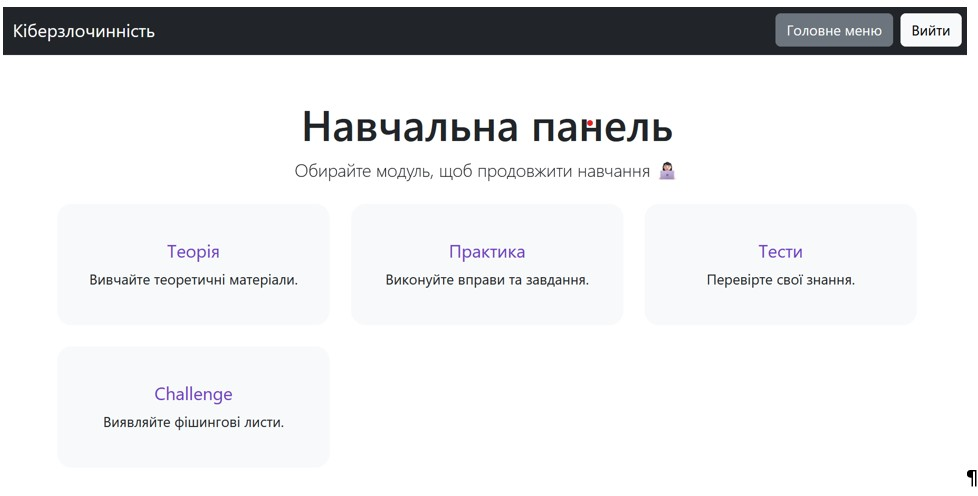
\includegraphics[width=0.98\linewidth]{img/figure6_1.jpg} 
    \caption{Інтерфейс головної панелі платформи для комплексного тренування навичок <<Cyber Simulator>>}
    \label{fig:6_1}
\end{figure}

Головна панель тренажера (рис.~\ref{fig:6_1}) надає користувачу швидкий доступ до симуляцій різних типів атак — від фішингу до SQL-ін’єкцій, дозволяючи візуалізувати власний прогрес та ідентифікувати слабкі місця у своїй системі знань.

\section*{Правова відповідальність}

Важливо усвідомлювати, що створення, використання та розповсюдження вірусів, троянів чи шпигунського програмного забезпечення — це не просто технічне хуліганство, а серйозна кримінальна діяльність, яка в Україні жорстко регулюється законом.

Дії зловмисників кваліфікуються за низкою статей Кримінального кодексу України~\cite{KKU2001}:
\begin{itemize}
    \item \textbf{Ст. 361.} Несанкціоноване втручання в роботу систем.
    \item \textbf{Ст. 361-1.} Створення та збут шкідливих програм.
    \item \textbf{Ст. 190.} Шахрайство.
\end{itemize}

Це означає, що за «легким заробітком» в інтернеті стоїть реальна кримінальна відповідальність. Правоохоронні органи мають інструменти для розслідування таких злочинів, спираючись як на національне законодавство, так і на міжнародну \textit{Конвенцію про кіберзлочинність}~\cite{Budapest_Convention_2001}.

Санкції за цими статтями передбачають суворе покарання, яке включає не лише значні штрафи та конфіскацію всіх програмних і технічних засобів, а й реальне позбавлення волі на тривалий термін.

\textit{\textbf{Важливо.} Окремо слід наголосити, що вчинення таких кіберзлочинів в умовах воєнного стану розглядається судом як обтяжуюча обставина, що значно посилює відповідальність. Тож розуміння природи шкідливого ПЗ потрібне не лише для захисту власних гаджетів, а й для усвідомлення правової межі, перетин якої перетворює користувача на злочинця.}

\section{Види шкідливих програм (віруси, трояни, шпигуни)}

\textbf{Шкідливе програмне забезпечення (ШПЗ, malware)} — це будь-які програми або код, створені з метою завдати шкоди користувачу, пристрою чи системі. Вони можуть блокувати роботу пристрою, викрадати дані або надавати зловмисникам несанкціонований доступ.

\vspace{0.3cm}

До основних типів шкідливих програм належать:

\begin{enumerate}
    \item \textbf{Програми-вимагачі (Ransomware).}
    Шкідливе ПЗ, яке шифрує або блокує файли й вимагає викуп за їх розблокування.
    \newline \textit{Приклад:} \textbf{WannaCry (2017)} — швидко зашифрував файли сотень тисяч ПК і вимагав платіж у біткоїнах.  

 \newpage

    \item \textbf{Трояни (Trojans).}
    Використовують візуальну ідентичність відомих брендів для вимкнення критичного сприйняття користувача, щоб непомітно виконувати шкідливі дії (приховано збирати персональні дані, перехоплювати управління пристроєм).
    \newline \textit{Приклад:} \textbf{Zeus} — перехоплював логіни в онлайн-банкінгу й виконував неавторизовані перекази.

    \item \textbf{Хробаки (Worms).}
    Поширюються мережею або через носії без участі користувача, часто викликають масові збої.
    \newline \textit{Приклад:} \textbf{SQL Slammer} — за кілька хвилин спричинив масштабні проблеми в мережах.

    \item \textbf{Рекламне ПЗ (Adware).}
    Нав’язливо показує рекламу, може перенаправляти на шахрайські сайти або змінювати налаштування браузера.
    \newline \textit{Приклад:} Кампанія \textbf{Fireball (2017)} — змінила стартові сторінки мільйонів комп'ютерів.

    \item \textbf{Ботнети\footnote{Мережа заражених пристроїв («зомбі»), якими керують зловмисники для виконання різних атак та злочинних дій.} (Botnets).}
    Мережі заражених пристроїв («зомбі»), якими керують зловмисники для DDoS-атак, розсилок або інших злочинних дій.
    \newline \textit{Приклад:} \textbf{Mirai (2016)} — DDoS-атаки з інфікованих IoT-пристроїв вивели з ладу великі сервіси. 

    \item \textbf{Шпигунське ПЗ (Spyware).}
    Непомітно збирає дані з пристрою: натискання клавіш, логіни й паролі, історію браузера, cookies, геолокацію, а інколи — аудіо чи відео; використовується для крадіжки облікових даних, банківської інформації або стеження. Основною метою цього класу програм залишається викрадення облікових даних та банківської інформації.
    
    Згідно з аналітичними даними компаній Check Point та Symantec, у 2023–2024 роках частка мобільного шпигунського ПЗ у загальній структурі шкідливих програм зросла з 12\% до 15\%. Експерти пов'язують цей тренд з еволюцією банківських троянів, які дедалі частіше інтегрують у себе шпигунські модулі для тотального контролю над інфікованим смартфоном~\cite{CheckPoint_2024, Symantec_Threat_2024}.

    \item \textbf{Руткіти\footnote{Програми, що надають зловмиснику прихований адміністративний доступ до системи та маскують свою присутність.} (Rootkits).}
    Програми, що надають зловмиснику прихований адміністративний доступ до системи. Відрізняються здатністю маскувати власну присутність та інше шкідливе ПЗ, що ускладнює виявлення.
    \newline \textit{Приклад:} \textbf{Stuxnet (2010)} — використовував руткіт-компоненти для приховування своєї присутності на заражених промислових системах.
\end{enumerate}

\subsection*{Ландшафт загроз 2024 року: Статистика та фінанси}

У 2024 році ландшафт кіберзагроз характеризувався чітким домінуванням шкідливого програмного забезпечення, орієнтованого на прихований контроль та прямий шантаж.

Статистичний аналіз інцидентів дозволяє виділити наступну структуру атак~\cite{AnyRun_Malware_2024}:

\begin{enumerate}
    \item \textbf{Троянські програми (Trojans).}
    Беззаперечний лідер загроз — зафіксовано близько \textbf{18 000} випадків, що становить \textbf{32\%} від загальної кількості атак. Це свідчить про те, що маскування під легітимне ПЗ залишається найефективнішим методом проникнення.

    \item \textbf{Програми-вимагачі (Ransomware).}
    Посіли друге місце з показником понад \textbf{12 000} інцидентів (\textbf{22\%}). Разом із троянами ці дві категорії сформували більше половини (54\%) усього вектора загроз.

    \item \textbf{Шпигунське ПЗ (Spyware).}
    Виявило значну активність — близько \textbf{9 000} випадків (\textbf{16\%}).
\end{enumerate}

Для розуміння природи загроз та методів протидії їм наведено детальну класифікацію шкідливого ПЗ (див. табл.~\ref{tab:table6_1}).

\begin{table}[H]
    \centering
    \footnotesize
    \caption{Класифікація шкідливого програмного забезпечення та особливості його роботи}
    \label{tab:table6_1}
    \renewcommand{\arraystretch}{1.05}
    \begin{tabular}{|>{\raggedright\arraybackslash}p{0.30\linewidth}|>{\raggedright\arraybackslash}p{0.30\linewidth}|>{\raggedright\arraybackslash}p{0.30\linewidth}|}
        \hline
        \multicolumn{1}{|c|}{\shortstack{\textbf{Вид шкідливого} \\ \textbf{ПЗ}}} & \multicolumn{1}{c|}{\shortstack{\textbf{Технічна} \\ \textbf{характеристика}}} & \multicolumn{1}{c|}{\shortstack{\textbf{Особливості} \\ \textbf{роботи}}} \\
        \hline
        \textbf{Програми-вимагачі} & Шифрування або блокування файлів системи & Монетизація через викуп (часто криптовалюта) \\
        \hline
        \textbf{Трояни} & Створення прихованого доступу (backdoor), крадіжка даних, доставка іншого ШПЗ & Маскування під легітимне ПЗ. Використовує механізми соціальної інженерії для стимулювання дії користувача \\
        \hline
        \textbf{Хробаки} & Перевантаження мережі, масове зараження & Самопоширення через мережеві вразливості. Не потребує дій користувача \\
        \hline
        \textbf{Рекламне ПЗ} & Показ нав'язливої реклами, редиректи, збір статистики & Встановлюється (часто приховано) разом з іншою програмою, яка завантажується \\
        \hline
    \end{tabular}
\end{table}



\begin{table}[H]
    \centering
    \footnotesize
    \caption*{Продовження таблиці 6.1}
    \renewcommand{\arraystretch}{1.05}
    \begin{tabular}{|>{\raggedright\arraybackslash}p{0.30\linewidth}|>{\raggedright\arraybackslash}p{0.30\linewidth}|>{\raggedright\arraybackslash}p{0.30\linewidth}|}
        \hline
        \multicolumn{1}{|c|}{\shortstack{\textbf{Вид шкідливого} \\ \textbf{ПЗ}}} & \multicolumn{1}{c|}{\shortstack{\textbf{Технічна} \\ \textbf{характеристика}}} & \multicolumn{1}{c|}{\shortstack{\textbf{Особливості} \\ \textbf{роботи}}} \\
        \hline
        \textbf{Ботнети} & Виконання команд (DDoS, спам, майнінг) & Централізоване управління мережею заражених пристроїв (зомбі-пристрої) \\
        \hline
        \textbf{Шпигунське ПЗ} & Крадіжка конфіденційної інформації (кейлоггінг, скріншоти, дані камери) & Прихована робота у фоновому режимі, моніторинг активності \\
        \hline
        \textbf{Віруси} & Пошкодження або модифікація файлів & Ін'єкція коду у легітимні файли. Потребує запуску файлу-носія для поширення \\
        \hline
        \textbf{Руткіти} & Надання повного (адміністративного) доступу до системи & Приховування присутності на рівні ядра ОС. Маскує файли, процеси та з'єднання \\
        \hline
    \end{tabular}
\end{table}

\textbf{Мобільний сегмент}
Окремий тренд спостерігається у мобільному сегменті: рекламне ПЗ (\textit{Adware}) та фейкові додатки сумарно охопили \textbf{21\%} ринку загроз (7 000 та 5 000 випадків відповідно). Менш чисельними, але стабільними загрозами залишилися ботнети (4 000) та комп'ютерні черв'яки (3 000), тоді як на специфічні інструменти (руткіти, криптоджекери) припало близько 4\% інцидентів.


\subsection*{Фінансовий моніторинг наслідків}

Фінансовий моніторинг наслідків кіберактивності у 2024 році демонструє чітку ієрархію загроз за рівнем монетизації.

\begin{itemize}
    \item \textbf{Ransomware.} Безумовний лідер за обсягом завданих збитків. Програми-вимагачі продемонстрували загрозливу динаміку зростання: щомісячні втрати постраждалих користувачів збільшилися майже вдвічі — з \$850 млн у січні до понад \textbf{\$1,5 млрд} у грудні.

    \item \textbf{Trojans.} Другу позицію у рейтингу фінансових загроз посіли троянські програми. Пік їхньої активності припав на серпень, коли сумарні збитки сягнули \textbf{\$1,25 млрд}, що пояснюється сезонними сплесками фішингових кампаній та відпустками персоналу служб безпеки.

    \item \textbf{Spyware.} Стабільно високий рівень фінансових втрат генерувало шпигунське ПЗ, збитки від якого наприкінці року оцінювалися в діапазоні \textbf{\$500--550 млн} щомісяця.

    \item \textbf{Фейкові мобільні додатки.} Аналітики відзначають тривожний тренд: якщо на початку року втрати становили \$180 млн, то у грудні цей показник зріс до \textbf{\$310 млн}, що корелює зі зростанням популярності мобільного банкінгу.
\end{itemize}



Інші вектори атак (рекламне ПЗ, черв'яки, ботнети), хоча й мали менший руйнівний потенціал, забезпечували постійний фон фінансових втрат у діапазоні \$100--300 млн на місяць.

\vspace{0.3cm}
\textit{Наведені оцінки базуються на крос-аналізі даних провідних галузевих звітів за 2024 рік: Check Point Cyber Security Report, Symantec Threat Landscape Report, Europol IOCTA, Chainalysis Crypto Crime Report~\cite{CheckPoint_2024, Symantec_Threat_2024, Europol_IOCTA_2024, Chainalysis_Crypto_2024}.}

Різні типи вірусів використовують специфічні канали проникнення та мають свої пріоритетні мішені; цей взаємозв'язок деталізовано в таблиці~\ref{tab:table6_2}.

\begin{table}[H]
    \centering
    \footnotesize
    \caption{Вектори поширення та типові цілі шкідливого програмного забезпечення}
    \label{tab:table6_2}
    \renewcommand{\arraystretch}{1.05}
    \begin{tabular}{|>{\raggedright\arraybackslash}p{0.30\linewidth}|>{\raggedright\arraybackslash}p{0.30\linewidth}|>{\raggedright\arraybackslash}p{0.30\linewidth}|}
        \hline
        \multicolumn{1}{|c|}{\shortstack{\textbf{Вид шкідливого} \\ \textbf{ПЗ}}} & \multicolumn{1}{c|}{\shortstack{\textbf{Основні вектори} \\ \textbf{атаки}}} & \multicolumn{1}{c|}{\shortstack{\textbf{Типові} \\ \textbf{цілі}}} \\
        \hline
        \textbf{Програми-вимагачі} & Email-вкладення, експлойти\footnotemark[3]\ вразливостей, RDP-атаки\footnotemark[4], фішингові сайти & Великі організації, лікарні, муніципальні установи, критична інфраструктура \\
        \hline
        \textbf{Трояни} & Фішингові листи, завантаження з веб-сайтів, зламані програми, оновлення софту & Банківські дані, облікові записи, бізнес-інформація, особисті файли \\
        \hline
        \textbf{Хробаки} & Експлуатація мережевих вразливостей, USB-накопичувачі, незахищені мережеві порти & Корпоративні мережі, IoT-пристрої, застарілі системи без оновлень \\
        \hline
        \textbf{Рекламне ПЗ} & Bundling\footnotemark[5]\ з безкоштовним ПЗ, браузерні розширення, оманливі банери & Пересічні користувачі, власники веб-сайтів, онлайн-рекламодавці \\
        \hline
    \end{tabular}
\end{table}
\footnotetext[3]{Код для використання вразливостей системи.}
\footnotetext[4]{Атаки через протокол віддаленого робочого столу.}
\footnotetext[5]{Об'єднання кількох програм в один інсталяційний пакет.}

\begin{table}[H]
    \centering
    \footnotesize
    \caption*{Продовження таблиці 6.2} 
    \renewcommand{\arraystretch}{1.05}
    \begin{tabular}{|>{\raggedright\arraybackslash}p{0.30\linewidth}|>{\raggedright\arraybackslash}p{0.30\linewidth}|>{\raggedright\arraybackslash}p{0.30\linewidth}|}
        \hline
        \multicolumn{1}{|c|}{\shortstack{\textbf{Вид шкідливого} \\ \textbf{ПЗ}}} & \multicolumn{1}{c|}{\shortstack{\textbf{Основні вектори} \\ \textbf{атаки}}} & \multicolumn{1}{c|}{\shortstack{\textbf{Типові} \\ \textbf{цілі}}} \\
        \hline
        \textbf{Ботнети} & Заражені IoT-пристрої, брутфорс\footnotemark[6]\ паролів, експлойти маршрутизаторів & DDoS-атаки на сервіси, розсилка спаму, криптомайнінг \\
        \hline
        \textbf{Шпигунське ПЗ} & Підроблені мобільні додатки, зламані програми, фішинг, уразливості нульового дня\footnotemark[7] & Журналісти, активісти, політики, бізнес-конкуренти, приватні особи \\
        \hline
        \textbf{Віруси} & Email-вкладення, заражені документи Office, інфіковані USB-накопичувачі & Файли користувачів, системні файли, документи, мережеві ресурси \\
        \hline
        \textbf{Руткіти} & Експлойти операційних систем, зламані драйвери, фізичний доступ до системи & APT-атаки\footnotemark[8]\ на уряди, промислові системи, критична інфраструктура \\
        \hline
    \end{tabular}
\end{table}
\footnotetext[6]{Метод підбору паролів перебором усіх варіантів.}
\footnotetext[7]{Невідомі розробникам вразливості без виправлень.}
\footnotetext[8]{Тривалі цілеспрямовані кібератаки організованих груп.}

Щоб оцінити реальний масштаб проблеми та виявити домінуючі тенденції, проаналізуємо структуру кіберінцидентів за останній звітний період (див. рис.~\ref{fig:6_2}).

\begin{figure}[H]
    \centering
    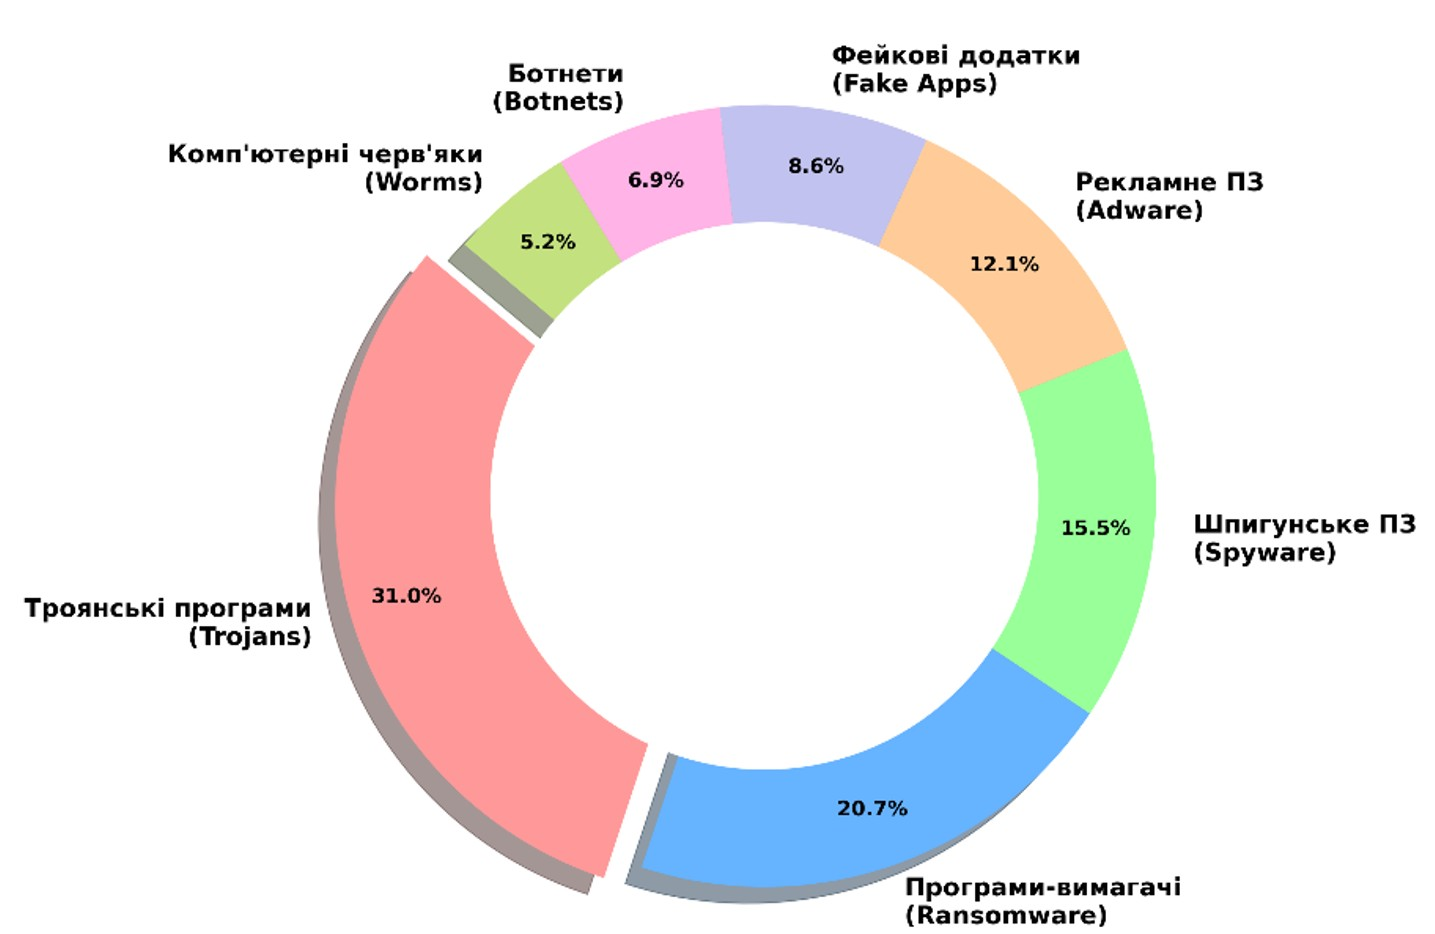
\includegraphics[width=0.90\linewidth]{img/figure6_2.jpg} 
    \caption{Структура кіберзагроз у 2024 році (розподіл за кількістю інцидентів)}
    \label{fig:6_2}
\end{figure}

\subsection*{Правова кваліфікація дій}

Правова кваліфікація дій, пов’язаних із розробкою та розповсюдженням шкідливого програмного забезпечення (зокрема фейкових мобільних додатків), в Україні здійснюється на основі норм Кримінального кодексу України (ККУ) та ратифікованих міжнародних договорів~\cite{KKU2001}.

До ключових статей, що інкримінуються у справах про кіберзлочини, належать:

\begin{description}
    \item[Ст. 361 ККУ.] «Несанкціоноване втручання в роботу інформаційних (автоматизованих), електронних комунікаційних, інформаційно-комунікаційних систем, електронних комунікаційних мереж». Ця стаття є базовою для кваліфікації злому систем та крадіжки даних.

    \newpage

    \item[Ст. 361-1 ККУ.] «Створення з метою протиправного використання, розповсюдження або збуту шкідливих програмних чи технічних засобів, а також їх розповсюдження або збут». Вона безпосередньо стосується розробників вірусів, троянів та програм-вимагачів.

    \item[Ст. 190 ККУ.] «Шахрайство». Застосовується (зокрема ч. 3 та ч. 4) у випадках заволодіння чужим майном шляхом обману з використанням електронно-обчислювальної техніки.

    \item[Ст. 200 ККУ.] «Незаконні дії з документами на переказ, платіжними картками та іншими засобами доступу до банківських рахунків». Ця норма регулює злочини у сфері електронного банкінгу (кардинг, скімінг).
\end{description}

Санкції за цими статтями передбачають значні штрафи, конфіскацію програмних та технічних засобів, а також позбавлення волі. Варто зазначити, що вчинення цих злочинів під час \textbf{воєнного стану} розглядається як обтяжуюча обставина.

Інтеграцію України у світову систему безпеки забезпечує \textit{Конвенція про кіберзлочинність} (Будапештська конвенція, 2001), ратифікована Верховною Радою у 2005 році. Цей документ уніфікує підходи до криміналізації розробки шкідливого ПЗ та створює правову основу для транскордонної співпраці правоохоронних органів у розслідуванні інтернет-злочинів~\cite{Budapest_Convention_2001}.


\section{Канали поширення через додатки та файли}

Канали поширення — це способи, якими шкідливе програмне забезпечення (ШПЗ) та фейкові мобільні додатки потрапляють на пристрої користувачів.

\newpage

До основних каналів належать:

\begin{enumerate}
    \item \textbf{Електронна пошта та веб-додатки.}
    Зараження через підозрілі покликання (фішинг) або шкідливі вкладення.

    \item \textbf{Завантаження з неофіційних джерел (Sideloading).}
    Встановлення мобільних додатків не з офіційних магазинів (Google Play, Apple App Store, Microsoft Store), а з веб-сайтів, форумів чи файлообмінників. Це основний шлях для потрапляння неперевіреного коду на пристрій.

    \item \textbf{Піратське ПЗ.}
    Розповсюдження «зламаних» (cracked) версій платних програм або інсталяторів, які маскуються під легітимне ПЗ, але модифіковані зловмисниками для прихованого встановлення вірусів.

    \item \textbf{Рекламні мережі (Malvertising).}
    Сторінки, які при перегляді веб-контенту автоматично перенаправляють користувача на небезпечні ресурси або завантажують шкідливий код.

    \item \textbf{Автоматичне зараження (Drive-by downloads).}
    Відбувається приховано під час відвідування скомпрометованого (легального, але зламаного) або спеціально створеного шахрайського веб-сайту.
\end{enumerate}

Такий поділ допомагає зрозуміти, якими шляхами зловмисники поширюють шкідливе ПЗ та на що слід звертати увагу.

\subsection*{Вектори атак у 2024 році}

У 2024 році архітектура вхідних точок для кібератак продемонструвала чітку специфіку залежно від сектору.

\newpage

\textbf{1. Корпоративний сектор}
Згідно зі звітом \textit{Verizon Data Breach Investigations Report (DBIR) 2024}, веб-додатки та електронна пошта залишаються головними векторами проникнення. Аналітики підкреслюють, що успішні атаки на веб-інтерфейси найчастіше реалізуються через два механізми: експлуатацію технічних вразливостей ПЗ або використання викрадених облікових даних \textit{<<Credential Stuffing>>} ~\cite{Verizon_DBIR_2024}.

\textbf{2. Мобільний сегмент}
Тут ключовою проблемою залишається завантаження програм із неофіційних джерел (\textit{sideloading}).

\begin{itemize}
    \item \textbf{Масштаб загрози.} За даними Google, система безпеки \textit{Google Play Protect} у 2024 році виявила понад \textbf{13 мільйонів} нових шкідливих застосунків, які намагалися встановитися поза межами офіційного магазину.
    \item \textbf{Джерело інфекції.} Статистика підтверджує небезпеку сторонніх джерел: понад \textbf{95\%} встановлень шкідливих програм, які зловживають критичними дозволами (доступ до SMS, контактів, фінансів), відбувалися через веб-браузери, файлові менеджери або месенджери, а не через Google Play Store~\cite{Google_BadApps_2024}.
    \item \textbf{Реакція екосистеми.} Протягом року Google заблокував публікацію 2,36 млн застосунків, що порушували політики безпеки, та забанив понад 158 000 акаунтів недобросовісних розробників.
\end{itemize}

Оскільки смартфони стали основними носіями конфіденційної інформації, зловмисники фокусують увагу саме на них. Візуалізацію ландшафту загроз для мобільних платформ наведено на рис.~\ref{fig:6_3}.

\begin{figure}[H]
    \centering
    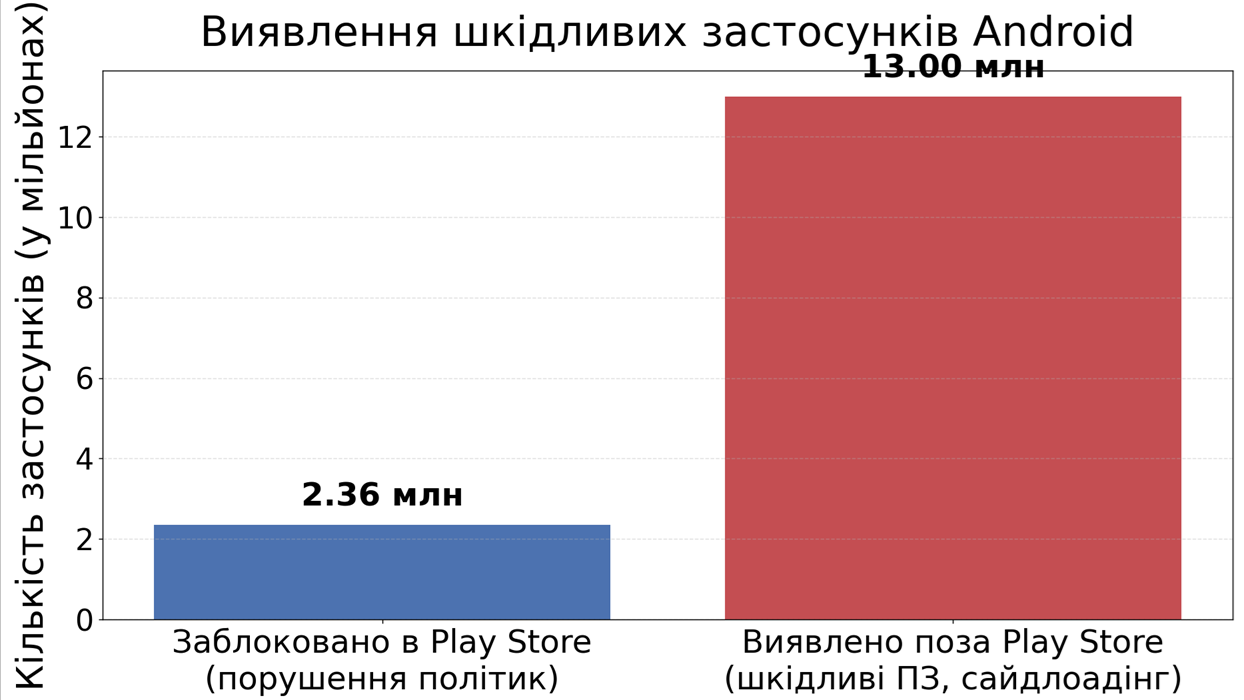
\includegraphics[width=0.99\linewidth]{img/figure6_3.png} 
    \caption{Візуалізація на мобільні пристрої)}
    \label{fig:6_3}
\end{figure}

\subsection*{Глобальний моніторинг: загрози sideloading}

Глобальний моніторинг мобільної безпеки підтверджує, що інсталяція додатків в обхід офіційних магазинів (\textit{sideloading}) є системною вразливістю екосистеми Android. Згідно зі звітом Zimperium «Global Mobile Threat Report 2024», саме цей вектор є джерелом значної частини інцидентів~\cite{Zimperium_Mobile_2024}.



\textbf{Географічний аналіз.}
Аналіз показує критичну ситуацію в Азійсько-Тихоокеанському регіоні, де близько \textbf{43\%} мобільних пристроїв мали встановлені застосунки з неофіційних джерел. Це створює сприятливе середовище для поширення:
\begin{itemize}
    \item мобільного шкідливого ПЗ (\textit{malware});
    \item рекламних вірусів (\textit{adware});
    \item кампаній з примусового встановлення небажаного софту.
  \end{itemize}

\newpage

\textbf{Масштаби протидії.}
Масштаби протидії цим загрозам ілюструють показники роботи системи \textit{Google Play Protect}: алгоритми захисту щодня сканують понад \textbf{200 мільярдів} застосунків, виконуючи глибинний аналіз на рівні коду для виявлення поліморфних загроз ще до їх активації на пристрої користувача (див. рис.~\ref{fig:6_4}).

\begin{figure}[H]
    \centering
    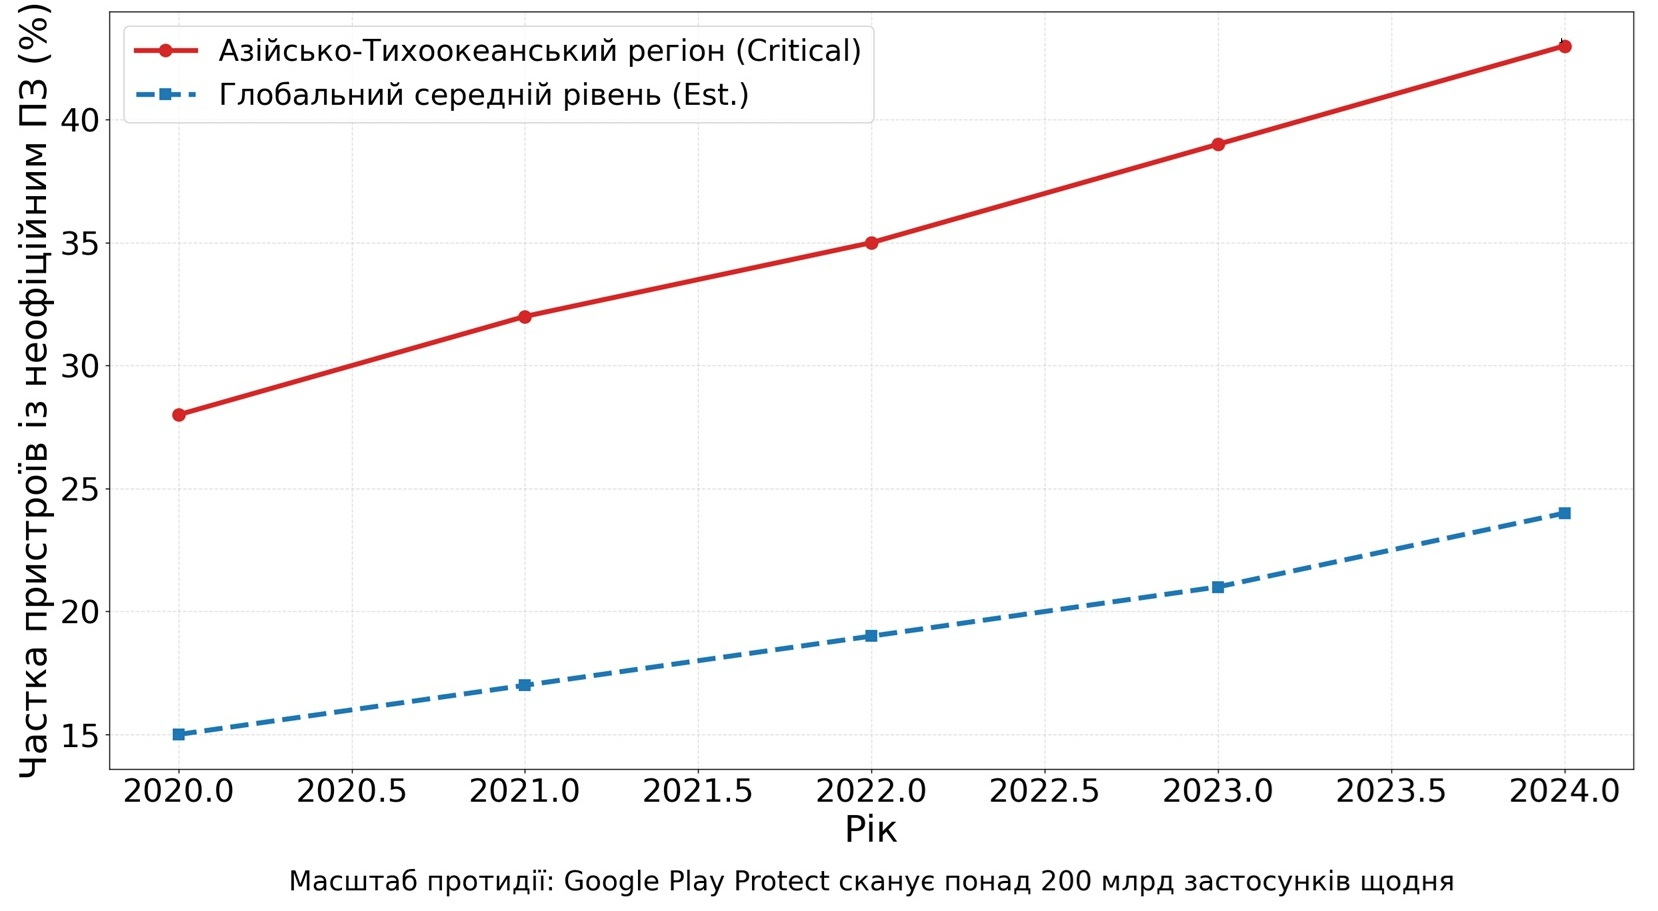
\includegraphics[width=0.90\linewidth]{img/figure6_4.jpg} 
    \caption{Динаміка вразливості екосистеми Android: Sideloading(Інсталяція додатків в обхід офіційних магазинів)}
    \label{fig:6_4}
\end{figure}

На рис.~\ref{fig:6_4} показано, звідки йдуть найбільші ризики. Щоб уникати їх, необхідно дотримуватися суворої цифрової гігієни:

\begin{itemize}
    \item \textbf{Не завантажувати} файли з підозрілих сайтів (особливо «зламані» програми).
    \item \textbf{Не відкривати} сумнівні покликання в SMS та чатах (навіть від знайомих).
    \item \textbf{Не відкривати} незнайомі вкладення в електронній пошті (архіви, офісні документи).
    \item \textbf{Не підключати} невідомі USB-накопичувачі до свого комп'ютера.
\end{itemize}

\newpage

Зловмисники адаптують свої інструменти під специфіку різних операційних систем. Співвідношення векторів поширення шкідливого ПЗ та їхніх цільових платформ показано на рис.~\ref{fig:6_5}.

\begin{figure}[H]
    \centering
    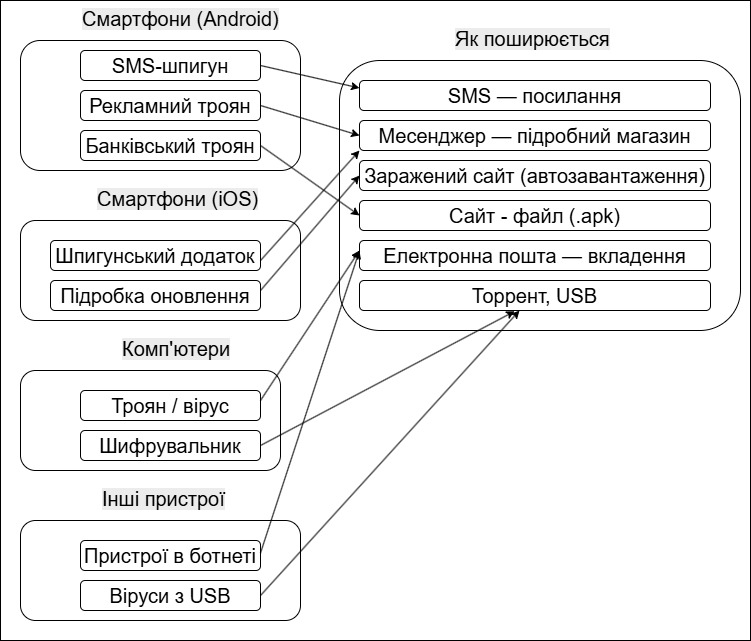
\includegraphics[width=0.80\linewidth]{img/figure6_5.jpg} 
    \caption{Вектори поширення шкідливого ПЗ та їх цільові платформи)}
    \label{fig:6_5}
\end{figure}

На схемі (див. рис.~\ref{fig:6_5}) показано, які пристрої найчастіше піддаються шкідливому ПЗ, які програми це ПЗ представляє і як воно потрапляє до користувачів.

\vspace{0.3cm}

\textbf{Структура схеми:}
\begin{itemize}
    \item \textbf{Зліва} позначені групи пристроїв: смартфони на Android, смартфони на iOS, комп’ютери та інші пристрої.
    \item \textbf{У середній частині} наведено приклади шкідливих програм для кожної групи — наприклад, банківські трояни, SMS-шпигуни, рекламні трояни, шифрувальники, віруси.

\newpage

    \item \textbf{Праворуч} показані звичайні шляхи поширення: завантаження файлів із веб-сайтів (\texttt{.apk} для Android), шкідливі покликання в SMS або чатах, підробні магазини додатків, вкладення в електронній пошті, торрент-файли, USB-накопичувачі та заражені сайти з автозавантаженням.
\end{itemize}

Стрілки на схемі ілюструють, який тип загрози найчастіше поширюється через конкретний канал — наприклад, банківський троян зазвичай приходить через файл із сайту, SMS-шпигун — через покликання в повідомленні, а шифрувальник — через піратські інсталятори або вкладення в листі.

\subsection*{Специфіка загроз за типом пристрою}

\begin{description}
    \item[Android-смартфони.]
    Основні загрози — банківські трояни, SMS-шпигуни та рекламні трояни. Вони поширюються переважно через неофіційні джерела: пряме завантаження \texttt{.apk} із сайтів, покликання у SMS або через підробні магазини додатків у месенджерах.

    \item[Смартфони на iOS.]
    Хоч і більш закриті, вони вразливі до шпигунських додатків та підроблених оновлень, які потрапляють через підробні магазини (з вимогою встановлення корпоративних профілів) або заражені веб-сайти з автоматичним завантаженням (\textit{drive-by}).

    \item[Комп’ютери.]
    Залишаються ціллю класичних троянів і вірусів, що найчастіше потрапляють через вкладення в електронній пошті. Шифрувальники та інше шкідливе ПЗ також активно поширюються через торрент-трекери або фізичні носії, такі як USB.
\end{description}

\section{Як працюють фейкові мобільні застосунки}

\textbf{Фейкові мобільні додатки} — це програми, які виглядають як знайомі сервіси (банк, маркетплейс, служба доставки або месенджер), але зроблені шахраями, щоб вкрасти ваші дані або гроші.

Вони копіюють логотипи й інтерфейс, щоб викликати довіру, і через це люди вводять логін, пароль або дані картки, думаючи, що користуються офіційною програмою.

\textbf{Механіка атаки.}
Всередині такі додатки приховують зловмисний код:
\begin{itemize}
    \item можуть показувати підробні вікна поверх справжніх банківських програм (так звані \textit{оверлеї});
    \item читати SMS з одноразовими кодами;
    \item збирати контакти та журнал дзвінків або відправляти інформацію на сервер шахраїв;
    \item іноді вони також запускають рекламу або використовують ресурси телефону для майнінгу (\textit{криптоджекінг}).
\end{itemize}

\subsection*{Як захиститися?}

Щоб не потрапити на шахраїв, дотримуйтесь наступних правил:
\begin{enumerate}
    \item \textbf{Завантажуйте програми тільки з офіційних магазинів} (Google Play, App Store).
    \item \textbf{Перевіряйте} ім’я розробника і відгуки перед встановленням.
    \item \textbf{Уважно дивіться}, які права (дозволи) просить додаток.
    \item \textbf{Не переходьте} за підозрілими покликаннями з SMS, чатів.
    \item \textbf{Використовуйте} мобільний захист (антивірус) за потреби.
\end{enumerate}

Для кращого розуміння алгоритму дій злочинців розглянемо типовий сценарій комплексної шахрайської схеми, який візуалізовано на рис.~\ref{fig:6_6}.

\begin{figure}[H]
    \centering
    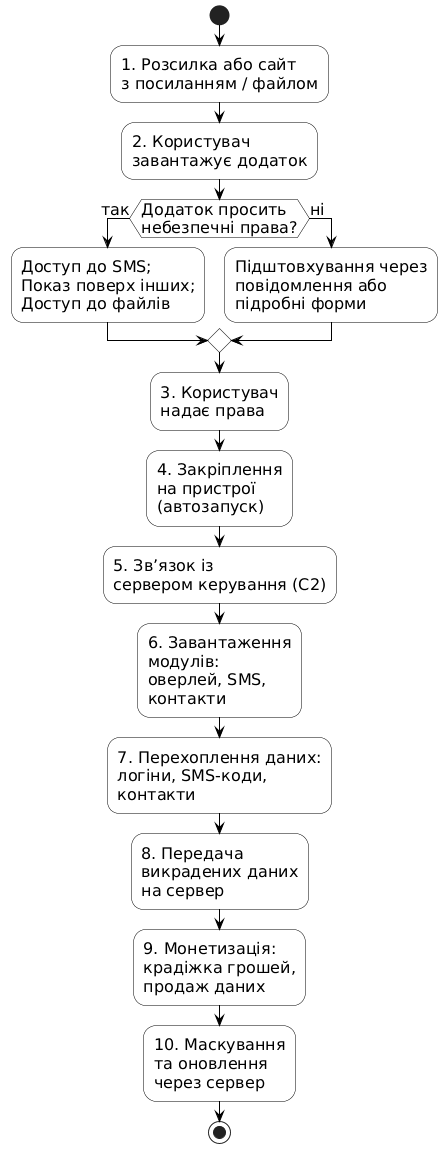
\includegraphics[width=0.45\linewidth]{img/figure6_6.png} 
    \caption{Сценарій небезпечних шахрайських схем}
    \label{fig:6_6}
\end{figure}

\newpage

Вищевказана схема показує спрощений сценарій атаки:

\begin{enumerate}
    \item \textbf{Доставка.} Шахрай розсилає покликання або підроблений додаток.
    \item \textbf{Інсталяція.} Користувач встановлює його і часто дає зайві права (дозволи).
    \item \textbf{Закріплення.} Програма закріплюється на пристрої, з'єднується з сервером шахрая (C2 server).
    \item \textbf{Виконання.} Підвантажує модулі для крадіжки даних і монетизації (гроші, файли, ботнет).
\end{enumerate}

Що стосується персональних комп'ютерів та серверів, спектр векторів атак є ширшим і включає складний фішинг, використання вразливостей операційних систем (експлойти) та Drive-by завантаження із заражених вебсайтів.

\subsection*{Приклад шахрайства: фейковий додаток (Львів)}

\textbf{Ситуація 1. Травень 2024 року}

Мешканець Львова, 42-річний приватний підприємець Андрій, о 10:12 отримав SMS-повідомлення з текстом: \textit{«Ваш рахунок заблоковано. Терміново підтвердьте доступ у застосунку»}.

\textbf{Соціальна інженерія.}
Відправником значився «MyBank Support», а в листі було покликання на сторінку з нібито офіційним мобільним додатком. Адреса виглядала переконливо — \texttt{https://mybannk-app.com/download}, де подвійна літера «n» була майже непомітною (тайпосквотинг). Переляк від можливої втрати доступу до рахунку після великого переказу змусив Андрія не звернути увагу на домен.

\newpage

\textbf{Технічна реалізація атаки.}
О 10:14 він завантажив установочний файл програми (файл із розширенням \texttt{.apk}\footnote{Формат файлу для встановлення додатків вручну на смартфон (ОС Android).}) і встановив додаток на свій Android-смартфон. Програма повністю імітувала офіційний банківський застосунок: логотип, кольори, меню входу.

Вже при запуску додаток попросив доступ до SMS та служби спеціальних можливостей (\textit{Accessibility Services}). Андрій погодився, не розуміючи ризиків.
Технічно це був банківський троян \textbf{«Xenomorph»}, який одразу почав:
\begin{itemize}
    \item перехоплювати одноразові коди з SMS;
    \item показувати фальшиві вікна для входу поверх справжнього застосунку банку (атака \textit{Overlay}).
\end{itemize}

\textbf{Фінансові та правові наслідки.}
О 10:19 з рахунку Андрія було здійснено три транзакції на загальну суму \textbf{147 000 грн}. Гроші спершу пішли на транзитний рахунок, а вже за кілька хвилин були переведені у криптовалюту.

\begin{itemize}
    \item \textbf{Економічно.} Андрій втратив місячний оборот бізнесу й був змушений оформити кредит для розрахунків із постачальниками. Банк відмовив у компенсації, оскільки клієнт самостійно встановив стороннє ПЗ.
    \item \textbf{Психологічно.} Він зазнав сильного стресу та почуття провини, вважаючи власну необережність причиною краху.
    \item \textbf{Юридично.} О 11:30 він подав заяву до кіберполіції; інцидент був кваліфікований за ст. 190 ККУ (шахрайство) та ст. 361 ККУ (несанкціоноване втручання в роботу комп’ютерних систем).
\end{itemize}

\newpage

\textit{\textbf{Висновки.} Цей випадок демонструє поєднання психологічного фактору (страх і терміновість) та технічної складової (фейковий .apk із правами Accessibility). Уникнути атаки можна було, якби Андрій завантажував застосунки лише з офіційного Google Play, перевірив адресу покликання та відмовився надавати критичні дозволи.}

\section{Додаткові приклади атак на смартфони}

Атаки на смартфони стали одними з найдинамічніших форм кіберзлочинності у 2024 році. За даними \textit{Google Threat Analysis Group}, понад \textbf{13 мільйонів} шкідливих застосунків було виявлено лише за один рік, а збитки користувачів від троянів, шпигунського ПЗ та програм-вимагачів на мобільних пристроях сягнули сотень мільйонів доларів.

\vspace{0.3cm}

\textbf{Типові сценарії прості:}
\begin{itemize}
    \item людина отримує SMS із покликанням на «оновлення банківського застосунку»;
    \item бачить рекламу у соцмережі з пропозицією завантажити «новий месенджер із функціями преміум»;
    \item знаходить «офіційний маркетплейс зі знижками».
\end{itemize}

Програма виглядає правдоподібно — знайомі кольори, логотипи, інтерфейс, але насправді містить троян чи шпигунський модуль. Після запуску вона запитує «звичайні» дозволи — доступ до SMS, геолокації, контактів чи мікрофона, і саме тут відбувається захоплення контролю.

\textit{Психологія працює на випередження:} поспіх («терміново підтвердьте доступ»), приваблива вигода («знижка 50\%»), або соціальний доказ («цей додаток уже завантажили тисячі»). Користувач під тиском не перевіряє адресу сторінки чи видавця у Play Store.

\subsection*{Історія 1. Як шахраї вкрали гроші: Історія Дмитра}

У вівторок, 19 листопада 2024 року, о 07:58 ранку мешканець Полтави Дмитро (31-річний інженер) отримав у Viber підозріле повідомлення. Воно було нібито від «підтримки банку “Обрій”» і вимагало «терміново перевірити пристрій», пропонуючи натиснути кнопку «Оновити додаток».

\textbf{Крок 1. Маскування під звичний інтерфейс}

покликання вело на сторінку, яка ідеально копіювала офіційний магазин Google Play, але адреса сайту була \texttt{obriy-app.com} — це була підробка, а не справжній сайт Google.

О 08:00 Дмитро натиснув «завантажити». Телефон запитав, чи дозволити браузеру (Chrome) встановлювати програми з невідомих джерел. Дмитро погодився і встановив шкідливий файл:
\begin{itemize}
    \item \textbf{Файл:} \texttt{ObriySecure\_v2.1.apk} (12,4 МБ)
    \item \textbf{Пакет:} \texttt{com.obriy.secure.update}
    \item \textbf{Хеш SHA-256:} \texttt{a91f...d4c7}
\end{itemize}

\textbf{Крок 2. Експлуатація фактору поспіху та довіри}

Під час першого запуску фейкова програма попросила надати їй кілька критично небезпечних дозволів. Програма запевнила, що все це потрібно «щоб активувати захист від шахрайства». Дмитро поспішав на ранкову нараду (о 9:00) і, під тиском терміновості, на все погодився:

\begin{enumerate}
    \item \textbf{«Служби доступності» (Accessibility Service).} Це найголовніший дозвіл. Він дозволяє програмі бачити абсолютно все на екрані та навіть натискати кнопки замість користувача.
    \item \textbf{«Доступ до сповіщень».} Щоб читати текст усіх сповіщень (включно з push-кодами від банку).
    \item \textbf{«Показ поверх інших програм».} Щоб створювати вікна-перехоплювачі (або імітовані інтерфейси) поверх оригінальних програм (Overlay attack).
    \item \textbf{«Доступ до SMS».} Щоб читати повідомлення з кодами підтвердження.
\end{enumerate}

\textbf{Як спрацювала атака (Технічний аспект)}

Технічно це був банківський вірус (троян). Хронологія злочину:

\begin{enumerate}
    \item \textbf{Крадіжка пароля (08:05).} Коли Дмитро відкрив справжній додаток банку, шкідлива програма помітила це і, використавши право накладати вікна поверх інших програм, миттєво показала ідеально скопійовану форму входу. Дмитро ввів у неї логін і пароль, і ці дані одразу відправилися на сервер зловмисників.
    
    \item \textbf{Перехоплення кодів (08:07).} Зловмисники ініціювали вхід в онлайн ‑ банкінг. Банк надіслав SMS‑код і повідомлення додатка для підтвердження, але троян, маючи доступ до сповіщень і SMS, автоматично перехопив ці коди і переслав їх на сервер зловмисників. Дмитро міг навіть не помітити цих повідомлень, оскільки троян може їх приховувати.
\end{enumerate}

\textit{Аналіз інциденту показав, що шкідливий додаток зареєстрував службу спеціальних можливостей, мав права читати SMS, отримувати повідомлення, накладати вікна поверх інших програм і автозапускатися при увімкненні телефону. У мережевих журналах зафіксовано регулярні звернення до сервера зловмисників і передачу зашифрованих даних.}

\subsection*{Фінал історії Дмитра: наслідки та результат}

О 08:09 та 08:11 з рахунку Дмитра вкрали \textbf{107 500 грн} (трьома переказами). Дмитро помітив серію сповіщень про списання грошей лише о 08:12. Він спробував зайти у свій банківський додаток, але бачив лише нескінченне завантаження («крутилку») — це вірус блокував йому доступ, продовжуючи показувати фальшивий екран. О 08:20 він додзвонився в банк і заблокував картку, а о 09:10 звернувся до кіберполіції.

\textbf{Результат.} Банк відмовив у компенсації. Юридична причина: Дмитро самостійно встановив програму не з офіційного магазину і надав їй критичні дозволи, що дозволило вірусу перехопити дані. Однак важливо розуміти: дії Дмитра не були проявом "наївності". Зловмисники використали стан стресу (ранкова нарада) та техніку оверлею, яка робить підміну інтерфейсу майже невидимою для людського ока. Це була професійна атака на психіку, а не просто технічна помилка чи необачність. До вечора Дмитро повністю скинув свій телефон до заводських налаштувань, змінив усі паролі та назавжди вимкнув у налаштуваннях можливість інсталяції з невідомих джерел, трансформувавши цей болючий досвід у навичку усвідомленої цифрової безпеки

\subsection*{Історія 2. «Віддалена заміна SIM-картки» (SIM-swapping): як втратити номер за 3 хвилини}

Механізм цієї атаки ілюструє реальна схема соціальної інженерії, яка активно використовується шахраями в месенджерах. Був звичайний вівторок, обідня перерва. Андрій, менеджер з логістики, гортав стрічку новин, коли у Viber надійшло повідомлення. Контакт мав ім’я «Мар’яна Vodafone», аватар — знайомий червоно-білий логотип оператора, а поруч із назвою був синій значок, що імітував позначку офіційного акаунта (рис.~\ref{fig:6_7-1s}).

Текст повідомлення був дивним і загрозливим:
\textit{«Скріншот надамо — подальші кроки для продовження. Змінювати SIM не потрібно, оскільки система формує серійний номер SIM-карти, яка встановлена у смартфоні. Лише після продовження необхідно виконати перезавантаження смартфону».}

\begin{figure}[H]
    \centering
    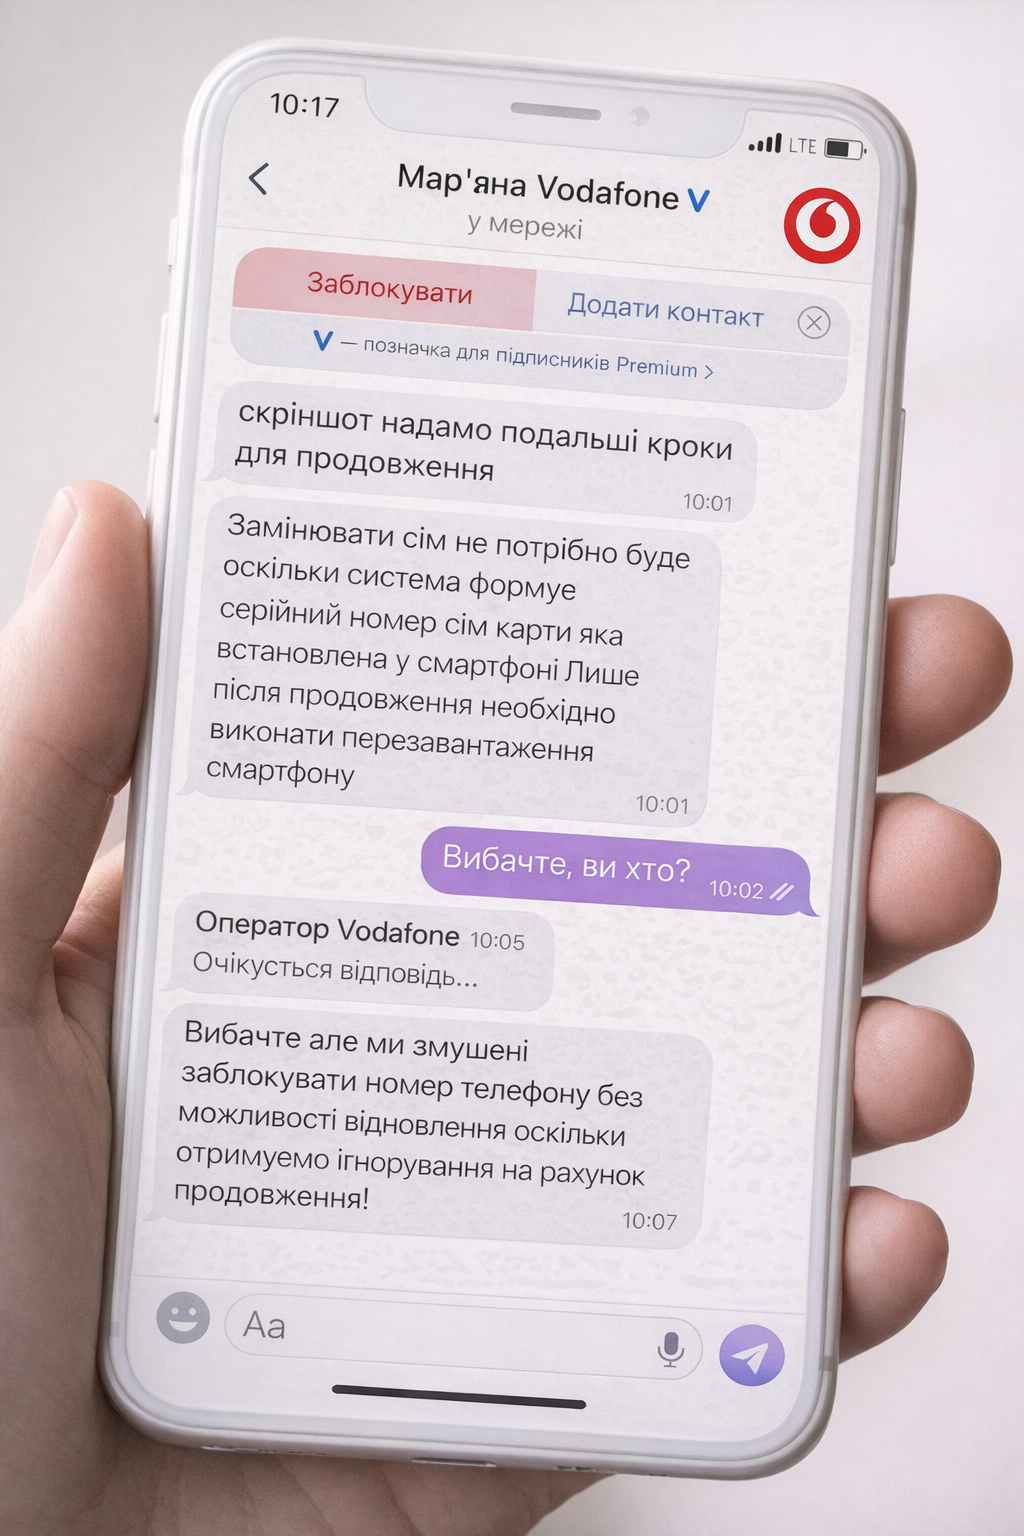
\includegraphics[width=0.75\linewidth]{img/fig6_7-1s.png}
    \caption{Приклад фейкового повідомлення від імені мобільного оператора у месенджері Viber}
    \label{fig:6_7-1s}
\end{figure}

Андрія насторожив тон повідомлення. Воно виглядало технічно й упевнено, але було плутаним. Він відповів коротко: \textit{«Вибачте, а ви хто?»}. 
Відповідь з’явилася майже одразу: \textit{«Оператор Vodafone»}.

Після цього співрозмовник написав: \textit{«Очікується відповідь»}, створюючи відчуття терміновості та контролю ситуації. Андрій не встиг нічого уточнити, як отримав нове повідомлення:

\textit{«Вибачте, але ми змушені заблокувати номер телефону без можливості відновлення, оскільки отримуємо ігнорування на рахунок продовження!»}

У цей момент Андрій відчув різкий страх. Цей номер був у нього 10 років: банки, пошта, робочі контакти, школа доньки — все було зав'язано на ньому. Втратити номер означало зупинити життя. Він швидко відповів: \textit{«Що мені робити? Я не можу їхати в салон, я на роботі».}

Відповідь прийшла миттєво: \textit{«Ми розуміємо. Для зручності клієнтів процедуру спрощено. Ми згенерували для вас віртуальний слот. Вам потрібно лише підтвердити перехід в офіційному додатку My Vodafone. Це безкоштовно».}

Це заспокоїло Андрія. Шахраї не просили номер картки, CVV-код чи пароль від Приват24. Вони навіть не скидали підозрілих посилань. Вони просили зайти в \textbf{офіційний} додаток оператора. Що може бути безпечніше?

\textit{«Зайдіть у меню "Послуги" $\rightarrow$ "Заміна SIM". Введіть серійний номер нової картки: 89380...»} — дбайливо інструктував «менеджер».

Андрій старанно виконав інструкції. Додаток запитав SMS-код для підтвердження заміни. 
— \textit{«Код прийшов. Вводити?»} — запитав Андрій у чаті.
— \textit{«Так, це фінальний крок для захисту номера».}

Він ввів код. На екрані з'явилося: «Заявку прийнято».

Через кілька хвилин зв’язок на телефоні зник. Індикатор мережі змінився на символ відсутності сигналу. «Мабуть, перезавантажується», — подумав Андрій і перезапустив пристрій. Але зв'язок не з'явився.

Вже через 5 хвилин Андрій спробував зайти в банківський застосунок Приват24 через Wi-Fi, щоб перевірити рахунок. Пароль не підходив. Доступ було втрачено. Він натиснув «Забули пароль?». При відновленні пароля система повідомила: \textit{«Код підтвердження надіслано на ваш номер»}. 

На номер, який вже працював в іншому телефоні під контролем зловмисників, за сотні кілометрів звідси. У цей момент Андрій усвідомив, що втратив не просто SIM-картку, а контроль над своєю цифровою ідентичністю.

\subsubsection*{Аналіз інциденту: чому схема спрацювала?}

Ця ситуація — класичний приклад соціальної інженерії, помноженої на довіру до офіційних інструментів.

\begin{enumerate}
    \item \textbf{Страх втрати.} Шахраї створили штучний дедлайн («номер буде заблоковано»), що відключило критичне мислення.
    \item \textbf{Ілюзія безпеки.} Жертву попросили скористатися офіційним додатком. Андрій думав, що якщо він у «рідній» програмі оператора, то йому нічого не загрожує. Він не знав, що функція «Заміна SIM» призначена для самостійної заміни картки на нову (яку ви купили в магазині), а не для «оновлення даних».
    \item \textbf{Підміна понять.} Вводячи серійний номер, який надіслали шахраї, Андрій фактично сказав системі: «Я купив нову SIM-картку (яка насправді вже була фізично у шахрая), перенесіть мій номер на неї».
\end{enumerate}

Злочинці використали техніку штучного прискореного зближення (rapid bonding), маскуючись під турботливу підтримку оператора. Використання офіційного додатка було лише способом знизити пильність. Це психологічна пастка: коли людина бачить знайомий логотип, її мозок автоматично переходить у режим довіри (валідація безпеки).

\subsection*{Інші сценарії атак}

\begin{description}
    \item[Історія 3. Фейковий банківський застосунок (Харків, 2024)]
    37‑річна вчителька Олена отримала SMS з покликанням на «оновлений додаток» банку. Встановила його (троян «Xenomorph»).
    \newline \textbf{Втрати:} 82 000 грн за 30 хвилин.
    \newline \textbf{Техніка.} Оверлей-атаки (фальшиві вікна поверх справжніх) + перехоплення SMS.

    \item[Історія 4. Фейковий маркетплейс (Київ, червень 2024)]
    29‑річний Максим встановив з Telegram «додаток знижок AliExpress» (.apk). Телефон почав показувати підроблені сторінки входу Google/Facebook.
    \newline \textbf{Втрати:} \$540 (викрадено дані карт з прив'язаних акаунтів).
    \newline \textbf{Техніка.} Фішинг-набір + MiTM-атака (перехоплення трафіку) + кейлогінг.

    \item[Історія 5. Фейковий месенджер (Одеса, вересень 2024)]
    18-річна Анна завантажила з сайту «YoWhatsApp» (мод месенджера). Додаток встановив троян \textit{Triada}, отримав root-права.
    \newline \textbf{Втрати:} 3 200 грн (приховані підписки на платні сервіси).
    \newline \textbf{Техніка.} Троян-завантажувач (Dropper), що діяв у фоновому режимі.

    \newpage

    \item[Історія 6. Фейковий криптогаманець (Дніпро, січень 2025)]
    34‑річний інвестор Ігор встановив з Google Play додаток-клона MetaMask. Після оновлення у ньому з’явився шкідливий код.
    \newline \textbf{Втрати:} 0,8 BTC (~1,3 млн грн) після введення seed-фрази.
    \newline \textbf{Техніка.} Атака на ланцюг поставок (\textit{supply-chain attack}) — чистий додаток стає шкідливим після апдейту.
\end{description}

\section*{Висновки}

Аналіз наведених випадків показує, що атаки через фейкові мобільні застосунки спираються на поєднання довіри користувачів до відомих брендів і технічних прийомів, які майстерно маскують справжню природу програми. Зловмисники копіюють логотипи, відтворюють інтерфейс і навіть іноді проходять початкову перевірку в офіційних магазинах, щоб створити ілюзію безпеки.

\textbf{Ключові фактори успіху атак:}
\begin{itemize}
    \item \textbf{Соціальна інженерія.} Користувачі надавали шкідливим програмам доступ, вважаючи це звичайною процедурою.
    \item \textbf{Технічна складність.} Використання оверлеїв, кейлогінгу та обходу двофакторної аутентифікації (2FA) через перехоплення SMS.
    \item \textbf{Безповоротність втрат.} Кошти швидко виводяться через транзитні рахунки та криптобіржі, що робить їх повернення майже неможливим.
\end{itemize}

Усі приклади доводять, що навіть ідеально схожий інтерфейс не гарантує безпеки. Лише поєднання уважності та базових навичок кібергігієни (завантаження тільки з офіційних сторів, перевірка дозволів) здатне зупинити атаку ще до введення даних.

\section{Ознаки зараження пристрою}

Якщо ви помітили ці ознаки, пам'ятайте: це не ваша вина. Сучасне шкідливе ПЗ розробляється так, щоб залишатися непомітним навіть для досвідчених користувачів. Ознаки зараження пристрою зазвичай проявляються поступово, але їх можна помітити, якщо уважно стежити за поведінкою смартфона чи комп’ютера.

Практичний аспект кібергігієни передбачає використання спеціалізованих інструментів для аналізу підозрілих файлів. Покрокові методи перевірки безпеки програм та інтерфейси відповідних сервісів детально проілюстровано на рис.~\ref{fig:6_7}--\ref{fig:6_16}.

\begin{figure}[H]
    \centering
    
\includegraphics[width=0.60\linewidth]{img/figure6_7.jpg} 
    \caption{Порівняння фейкового та справжнього сайту}
    \label{fig:6_7}
\end{figure}

\begin{figure}[H]
    \centering
    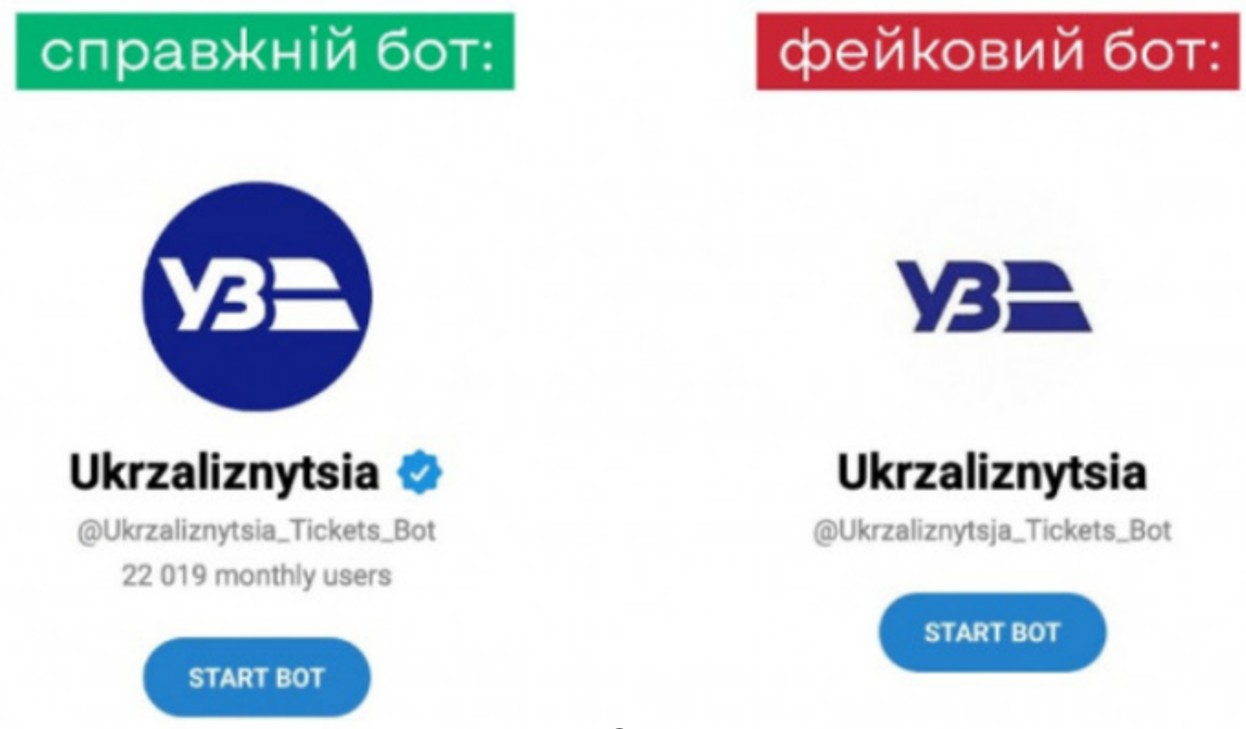
\includegraphics[width=0.80\linewidth]{img/figure6_8.jpg} 
    \caption{Порівняння фейкового та справжнього сайту}
    \label{fig:6_8}
\end{figure}

\begin{figure}[H]
    \centering
    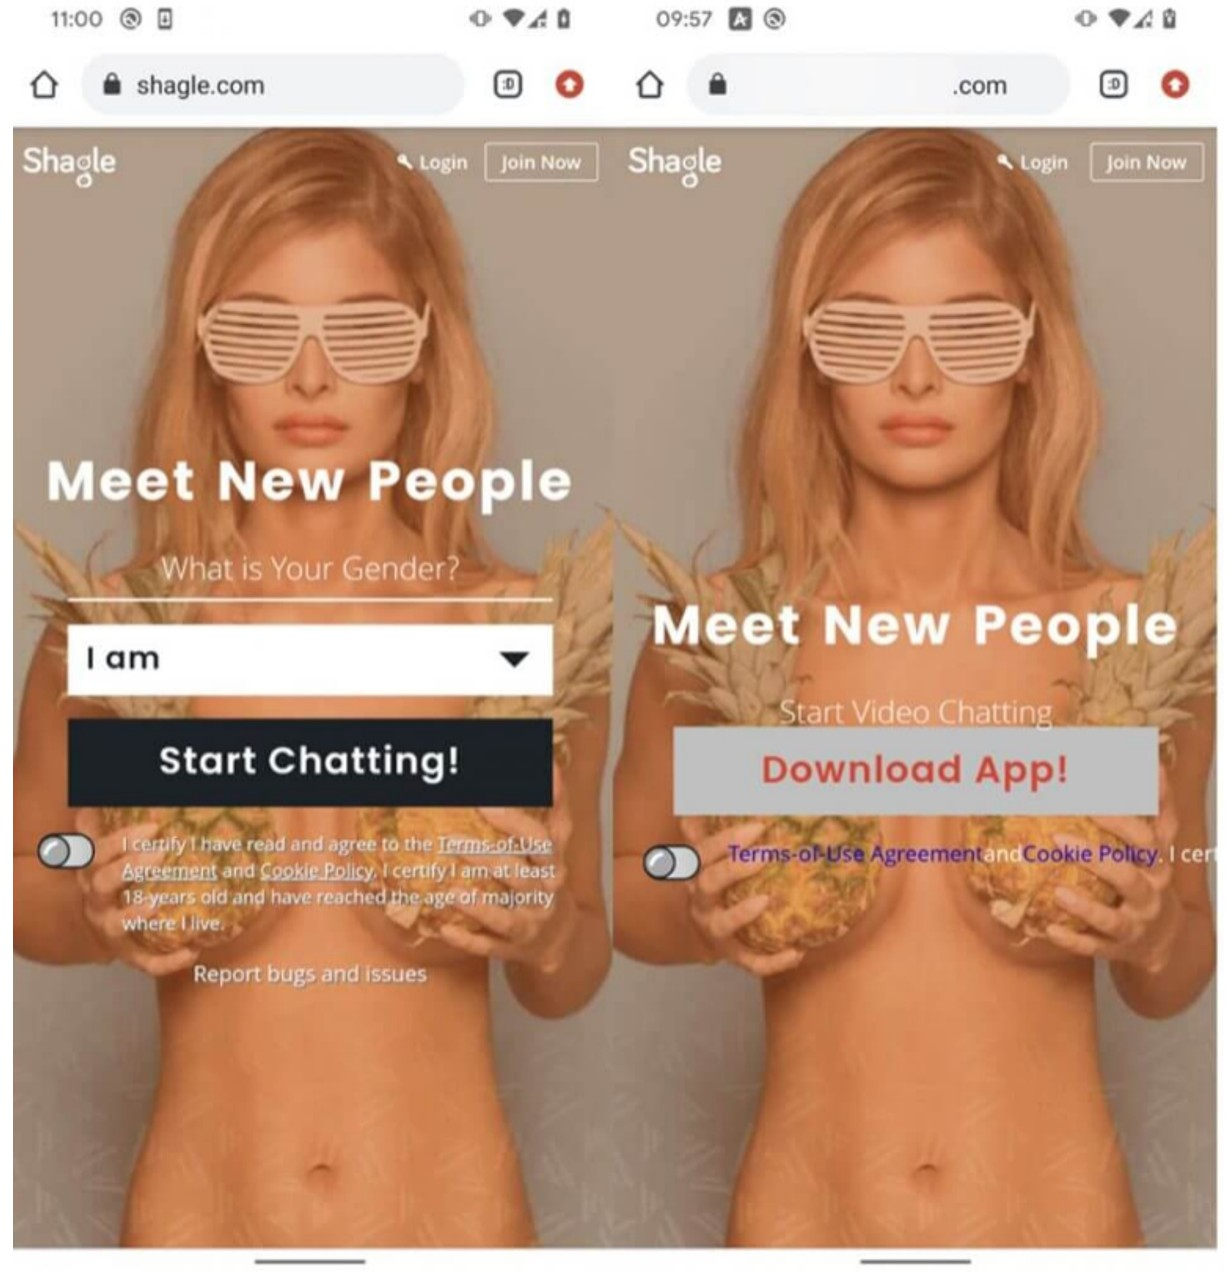
\includegraphics[width=0.90\linewidth]{img/figure6_9.jpg} 
    \caption{Аналіз справжніх додатків в GoogleStore}
    \label{fig:6_9}
\end{figure}

\begin{figure}[H]
    \centering
    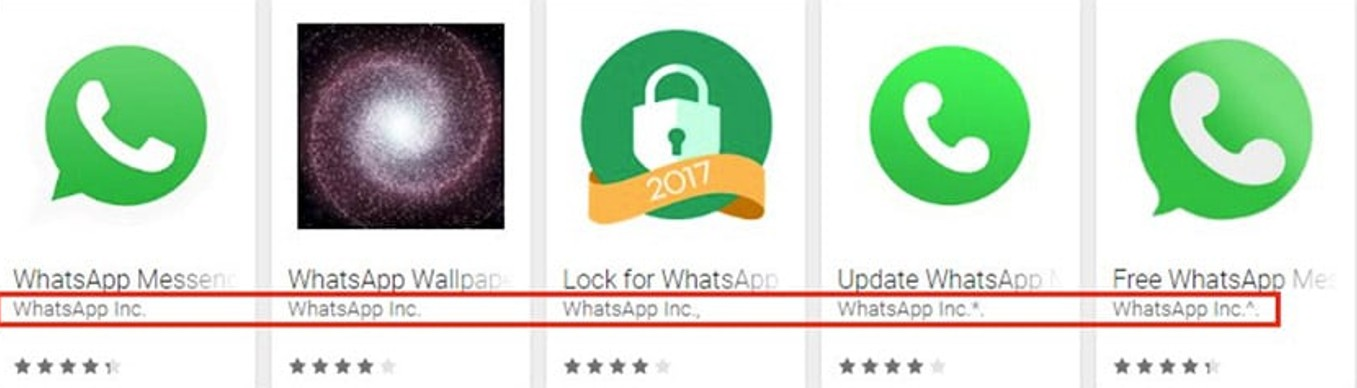
\includegraphics[width=0.90\linewidth]{img/figure6_10.jpg} 
    \caption{Порівняння фейкового та справжнього сайту}
    \label{fig:6_10}
\end{figure}

\begin{figure}[H]
    \centering
    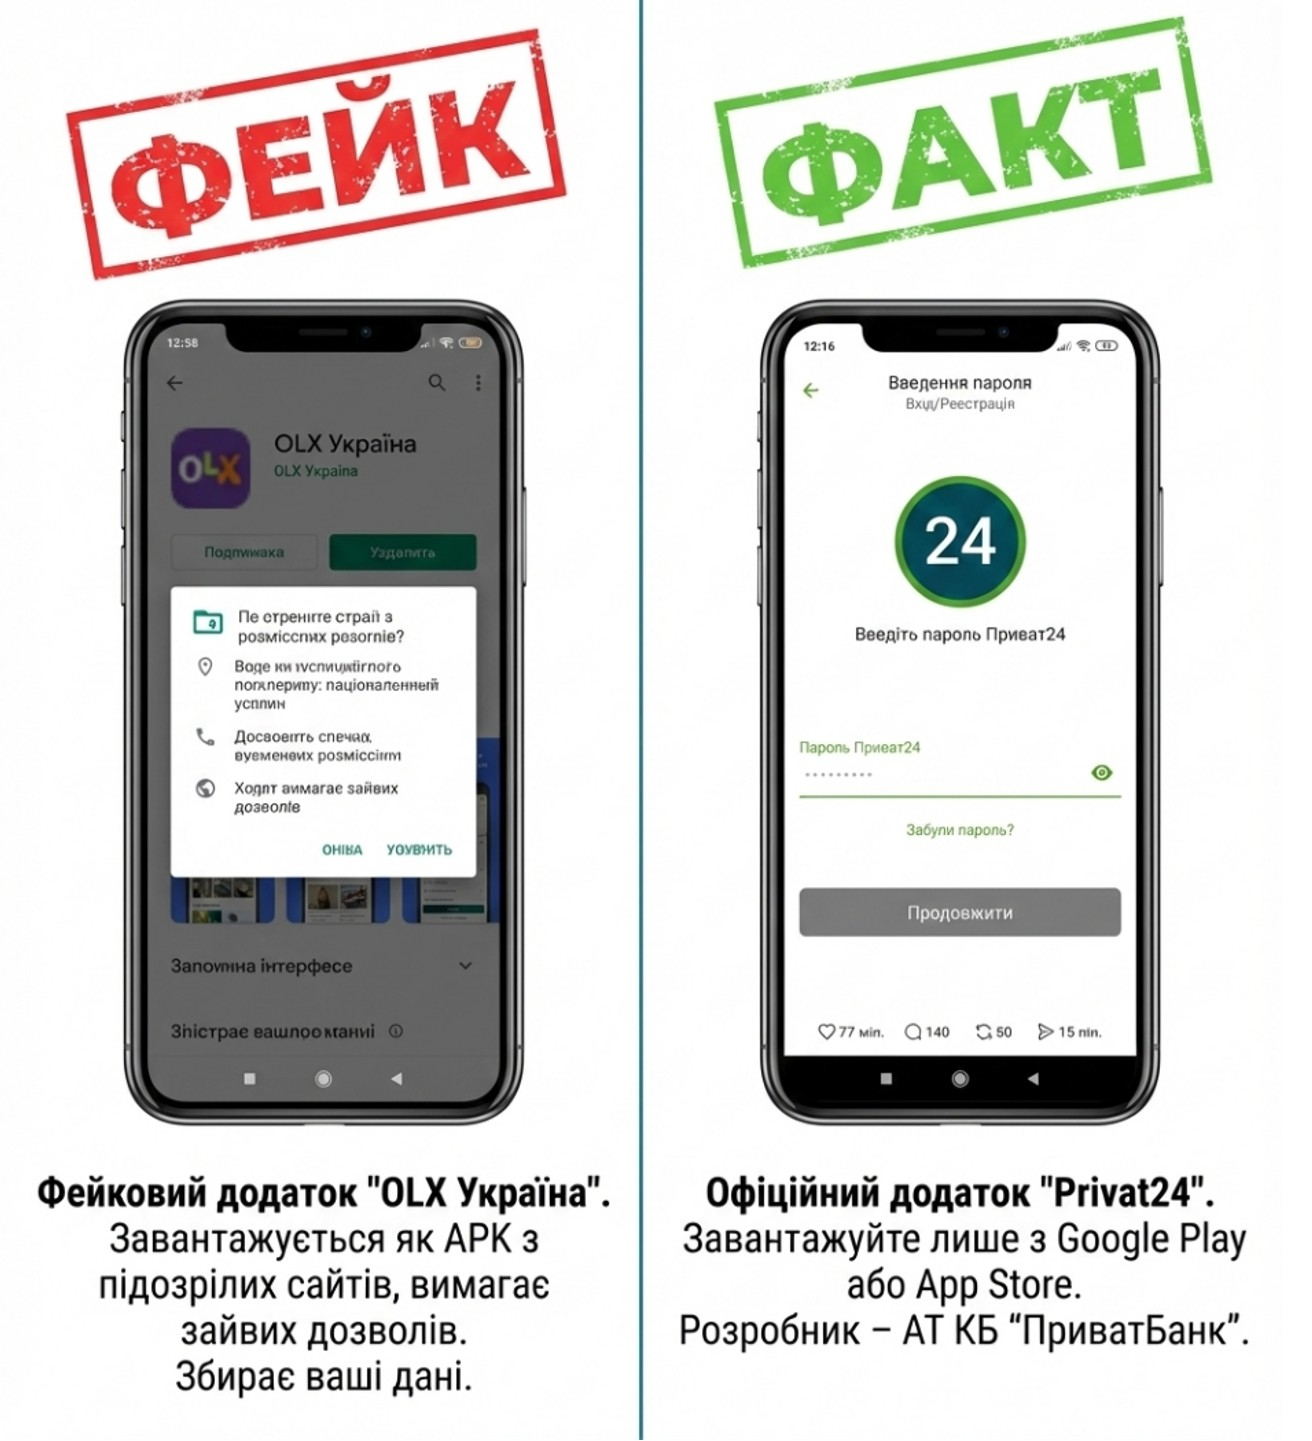
\includegraphics[width=0.60\linewidth]{img/figure6_11.jpg} 
    \caption{Порівняння фейкового та справжнього додатку}
    \label{fig:6_11}
\end{figure}

\begin{figure}[H]
    \centering
    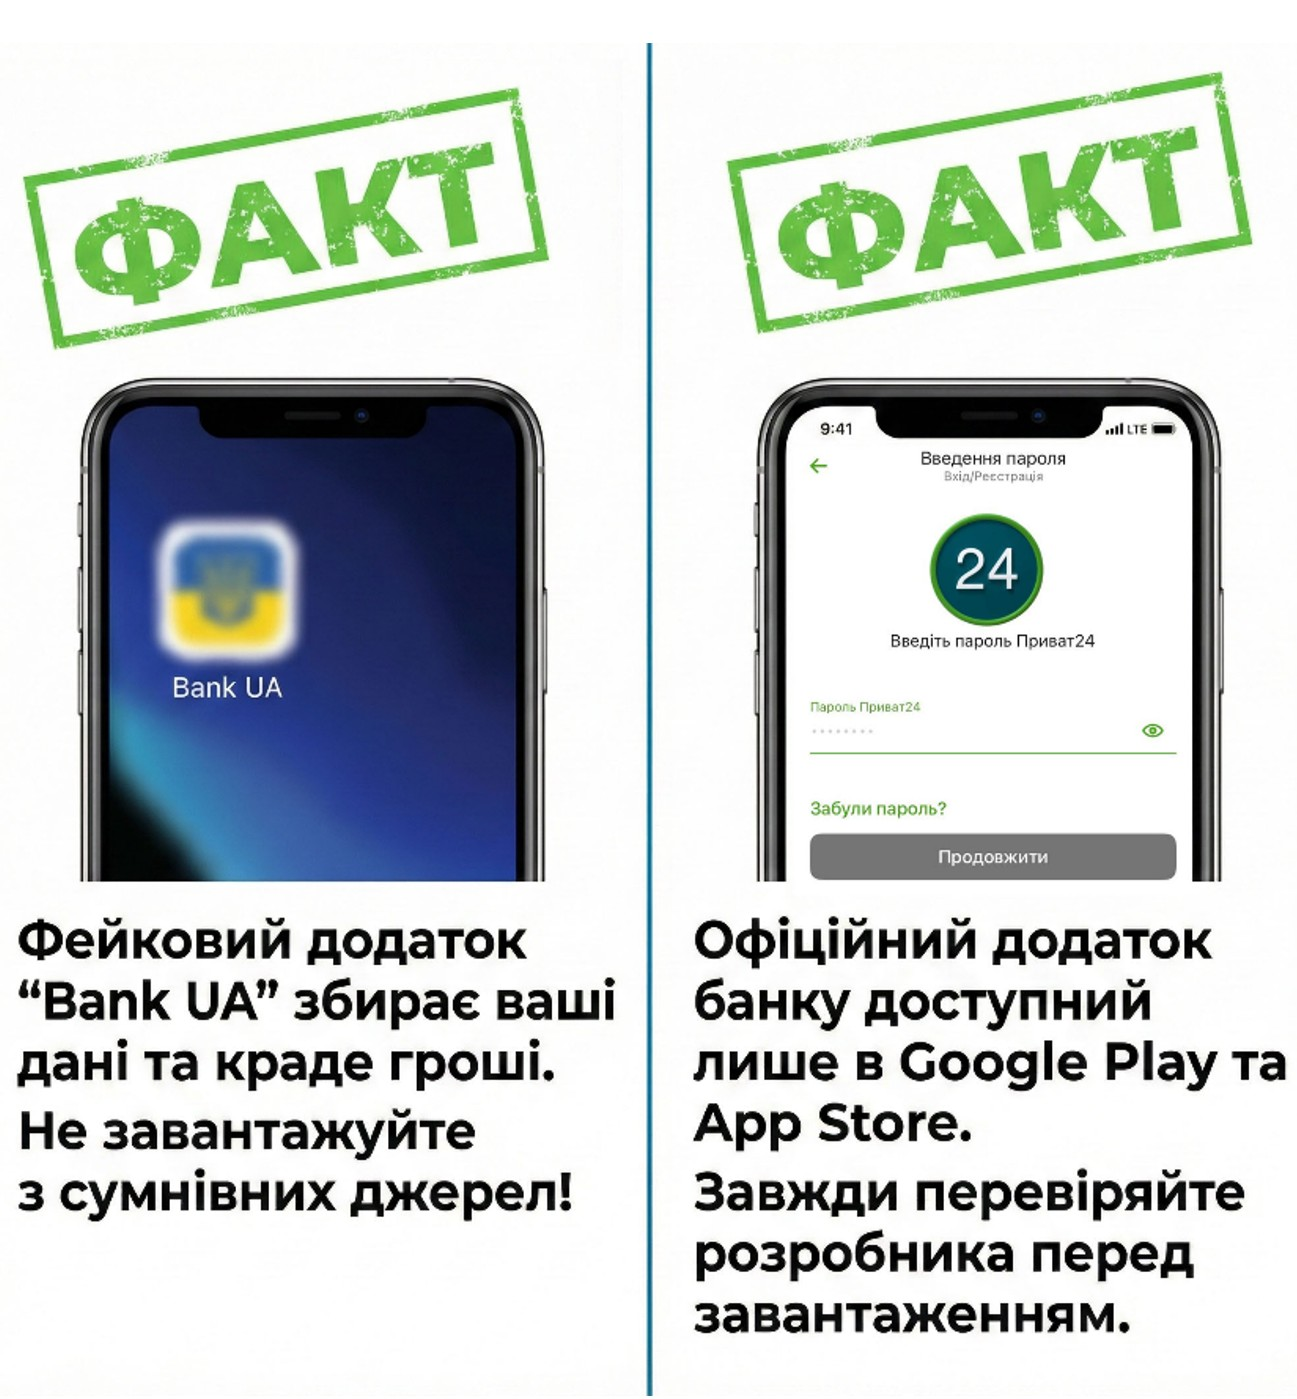
\includegraphics[width=0.60\linewidth]{img/figure6_12.jpg} 
    \caption{Листування щодо скачування фейкового додатку}
    \label{fig:6_12}
\end{figure}

\begin{figure}[H]
    \centering
    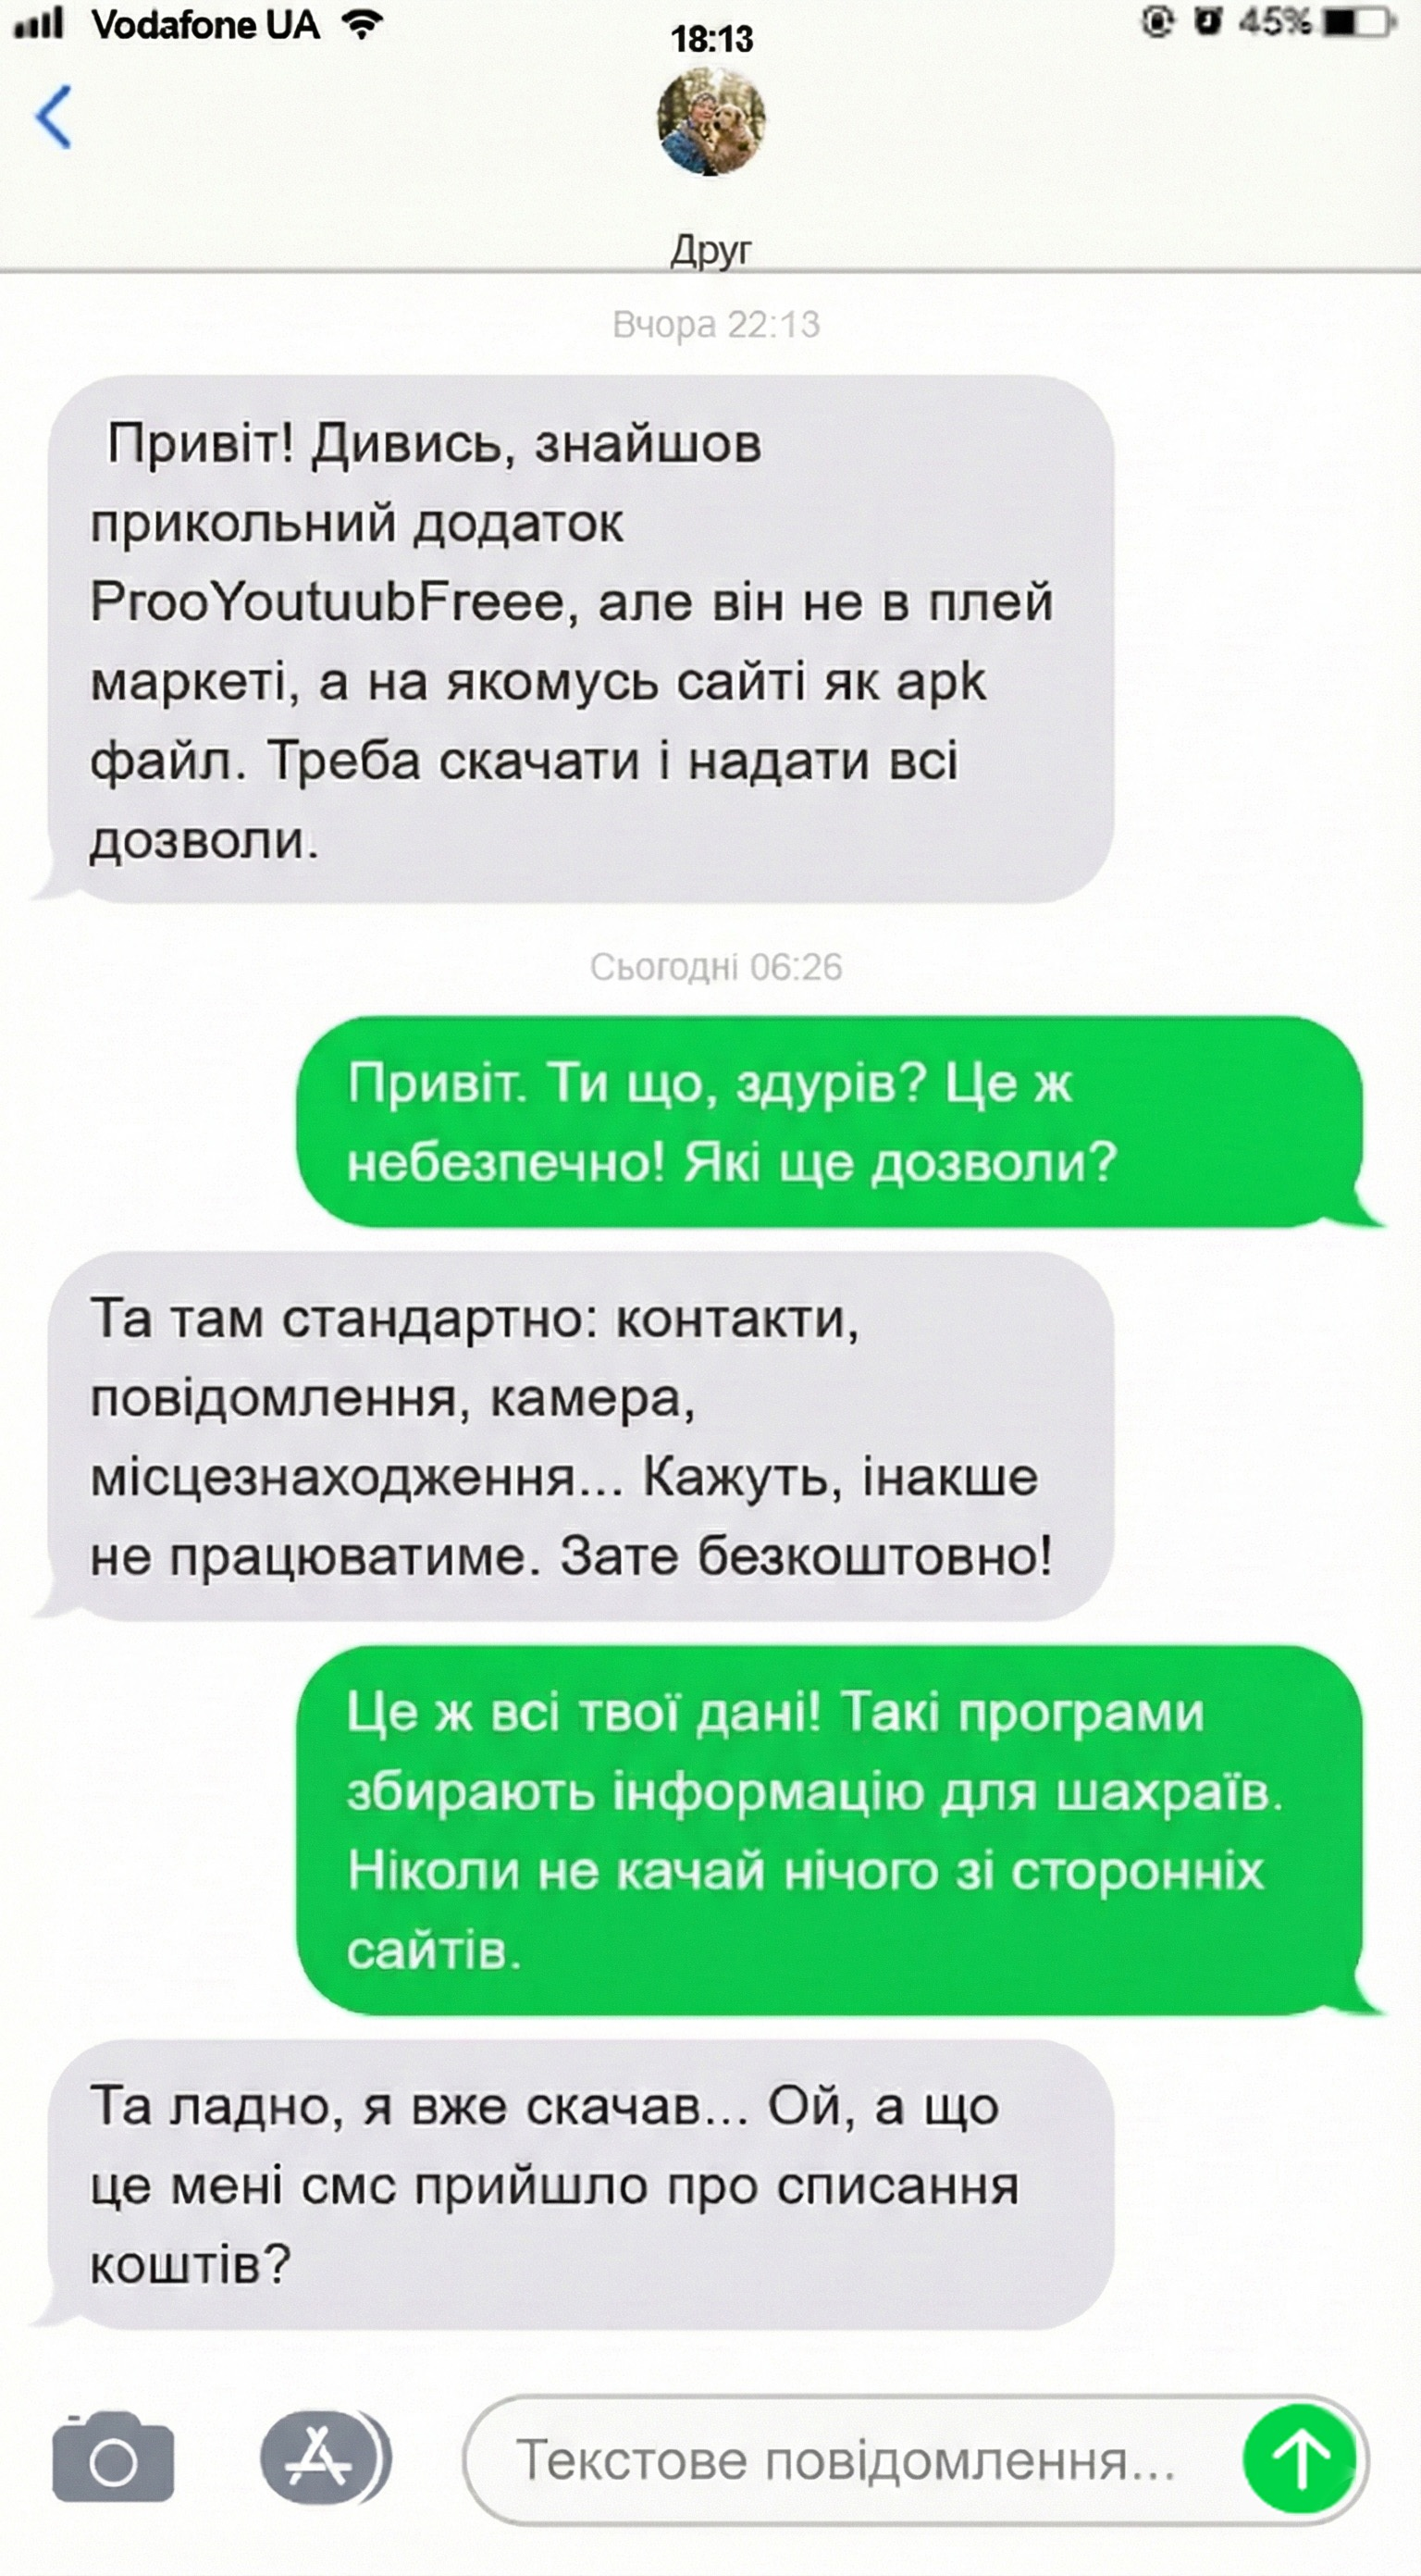
\includegraphics[width=0.70\linewidth]{img/figure6_13.jpg} 
    \caption{Листування з другом щодо скачування фейкового додатку}
    \label{fig:6_13}
\end{figure}

\begin{figure}[H]
    \centering
    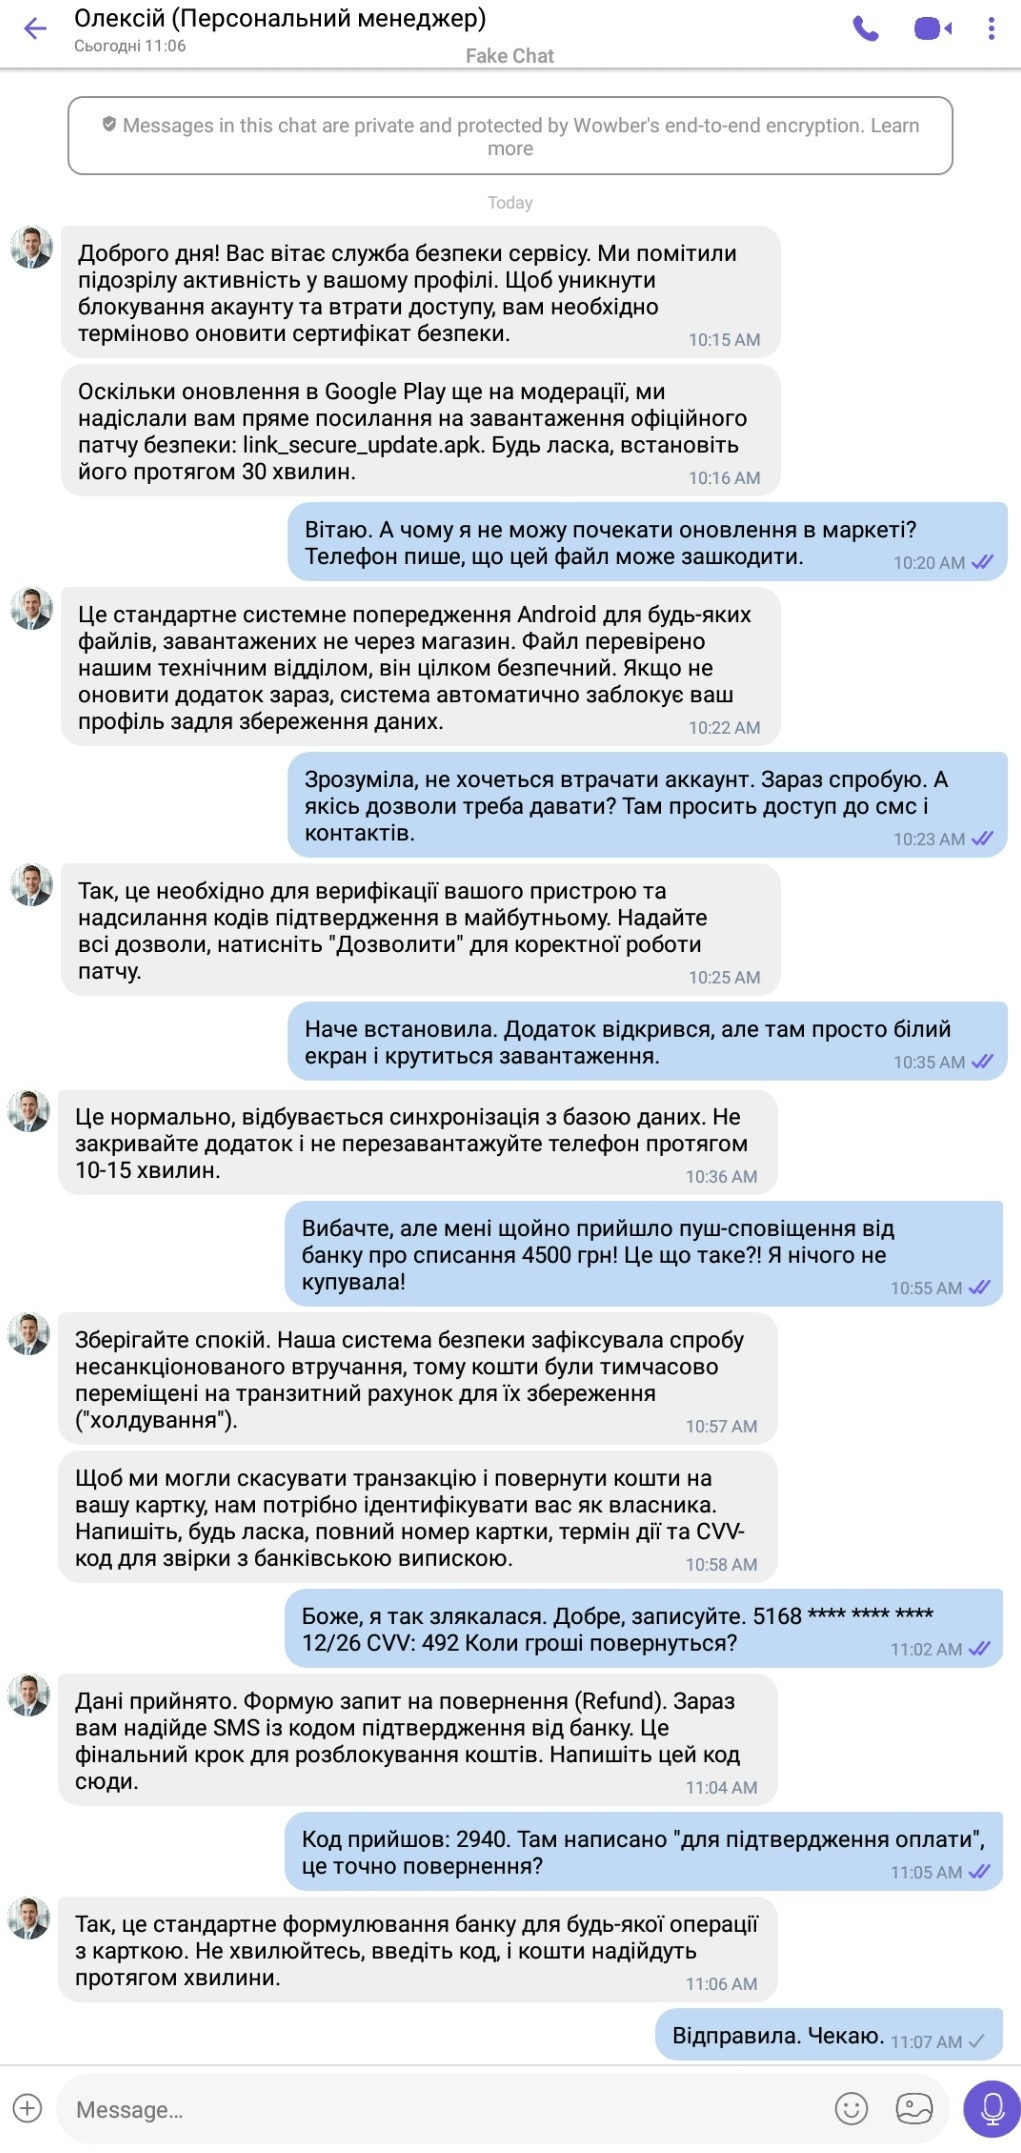
\includegraphics[width=0.70\linewidth]{img/figure6_14.jpg} 
    \caption{Листування щодо скачування фейкового додатку}
    \label{fig:6_14}
\end{figure}

\begin{figure}[H]
    \centering
    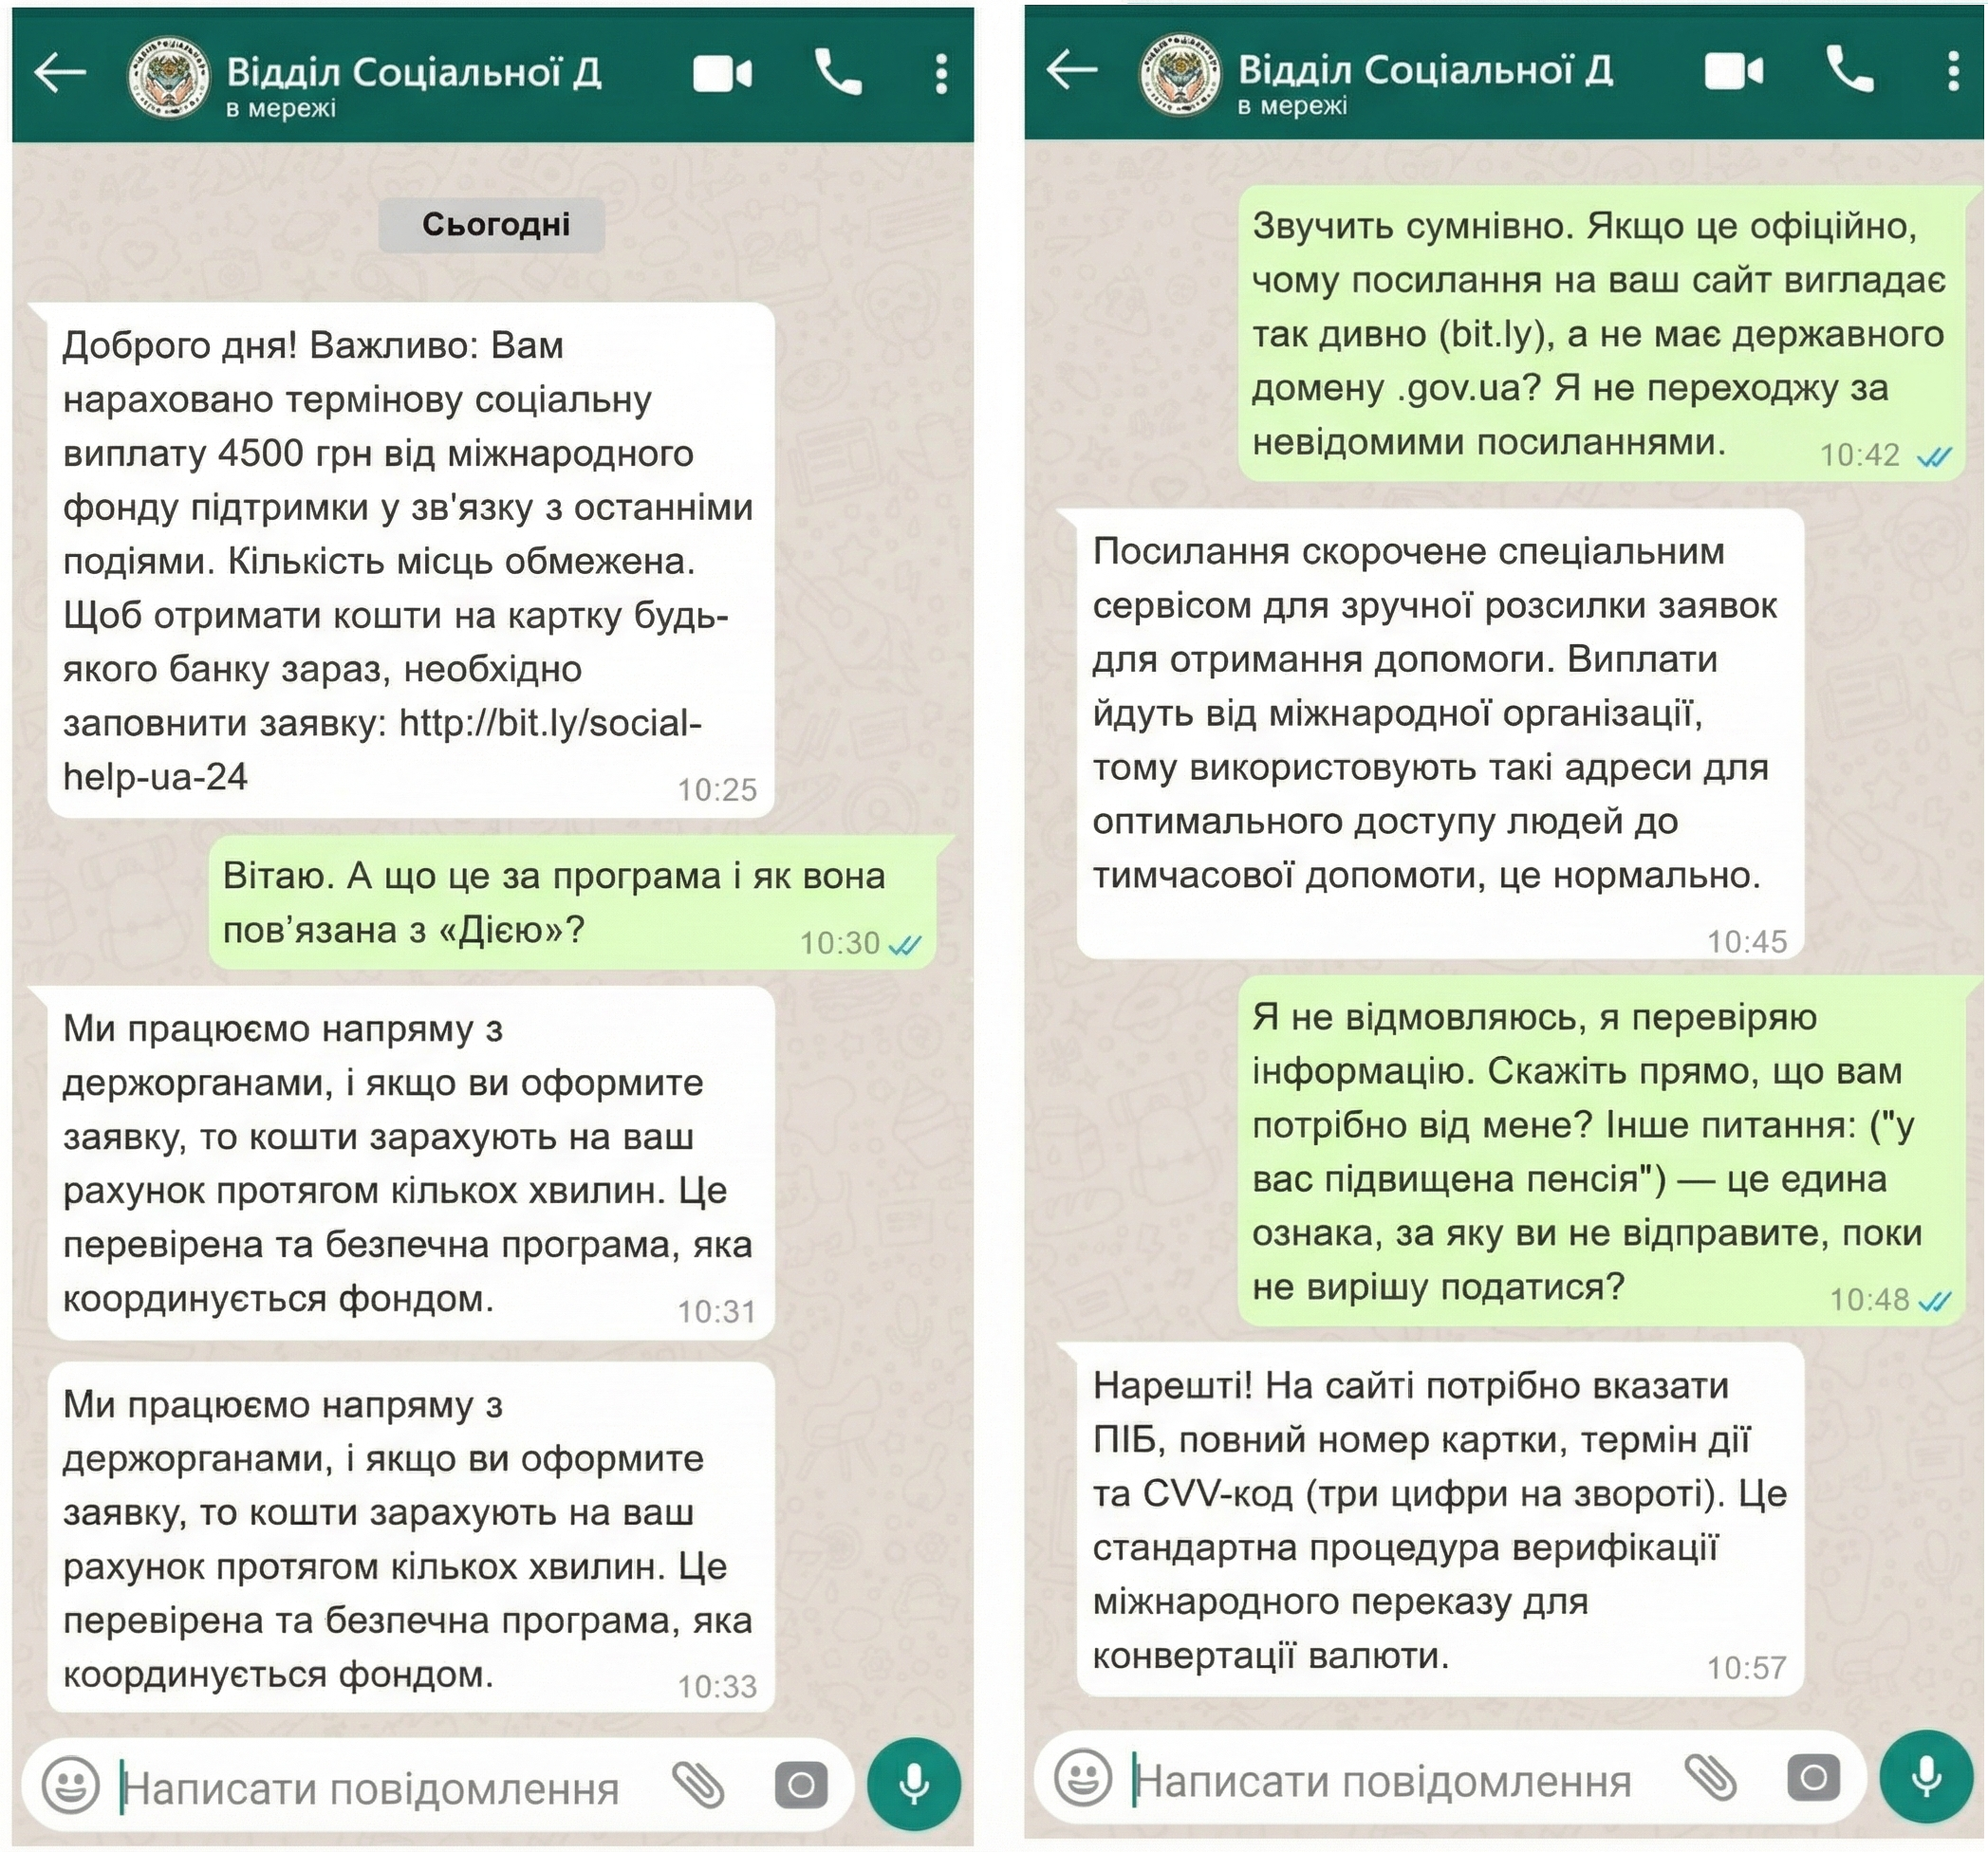
\includegraphics[width=0.75\linewidth]{img/figure6_15.png} 
    \caption{Листування щодо скачування фейкового додатку}
    \label{fig:6_15}
\end{figure}

\begin{figure}[H]
    \centering
    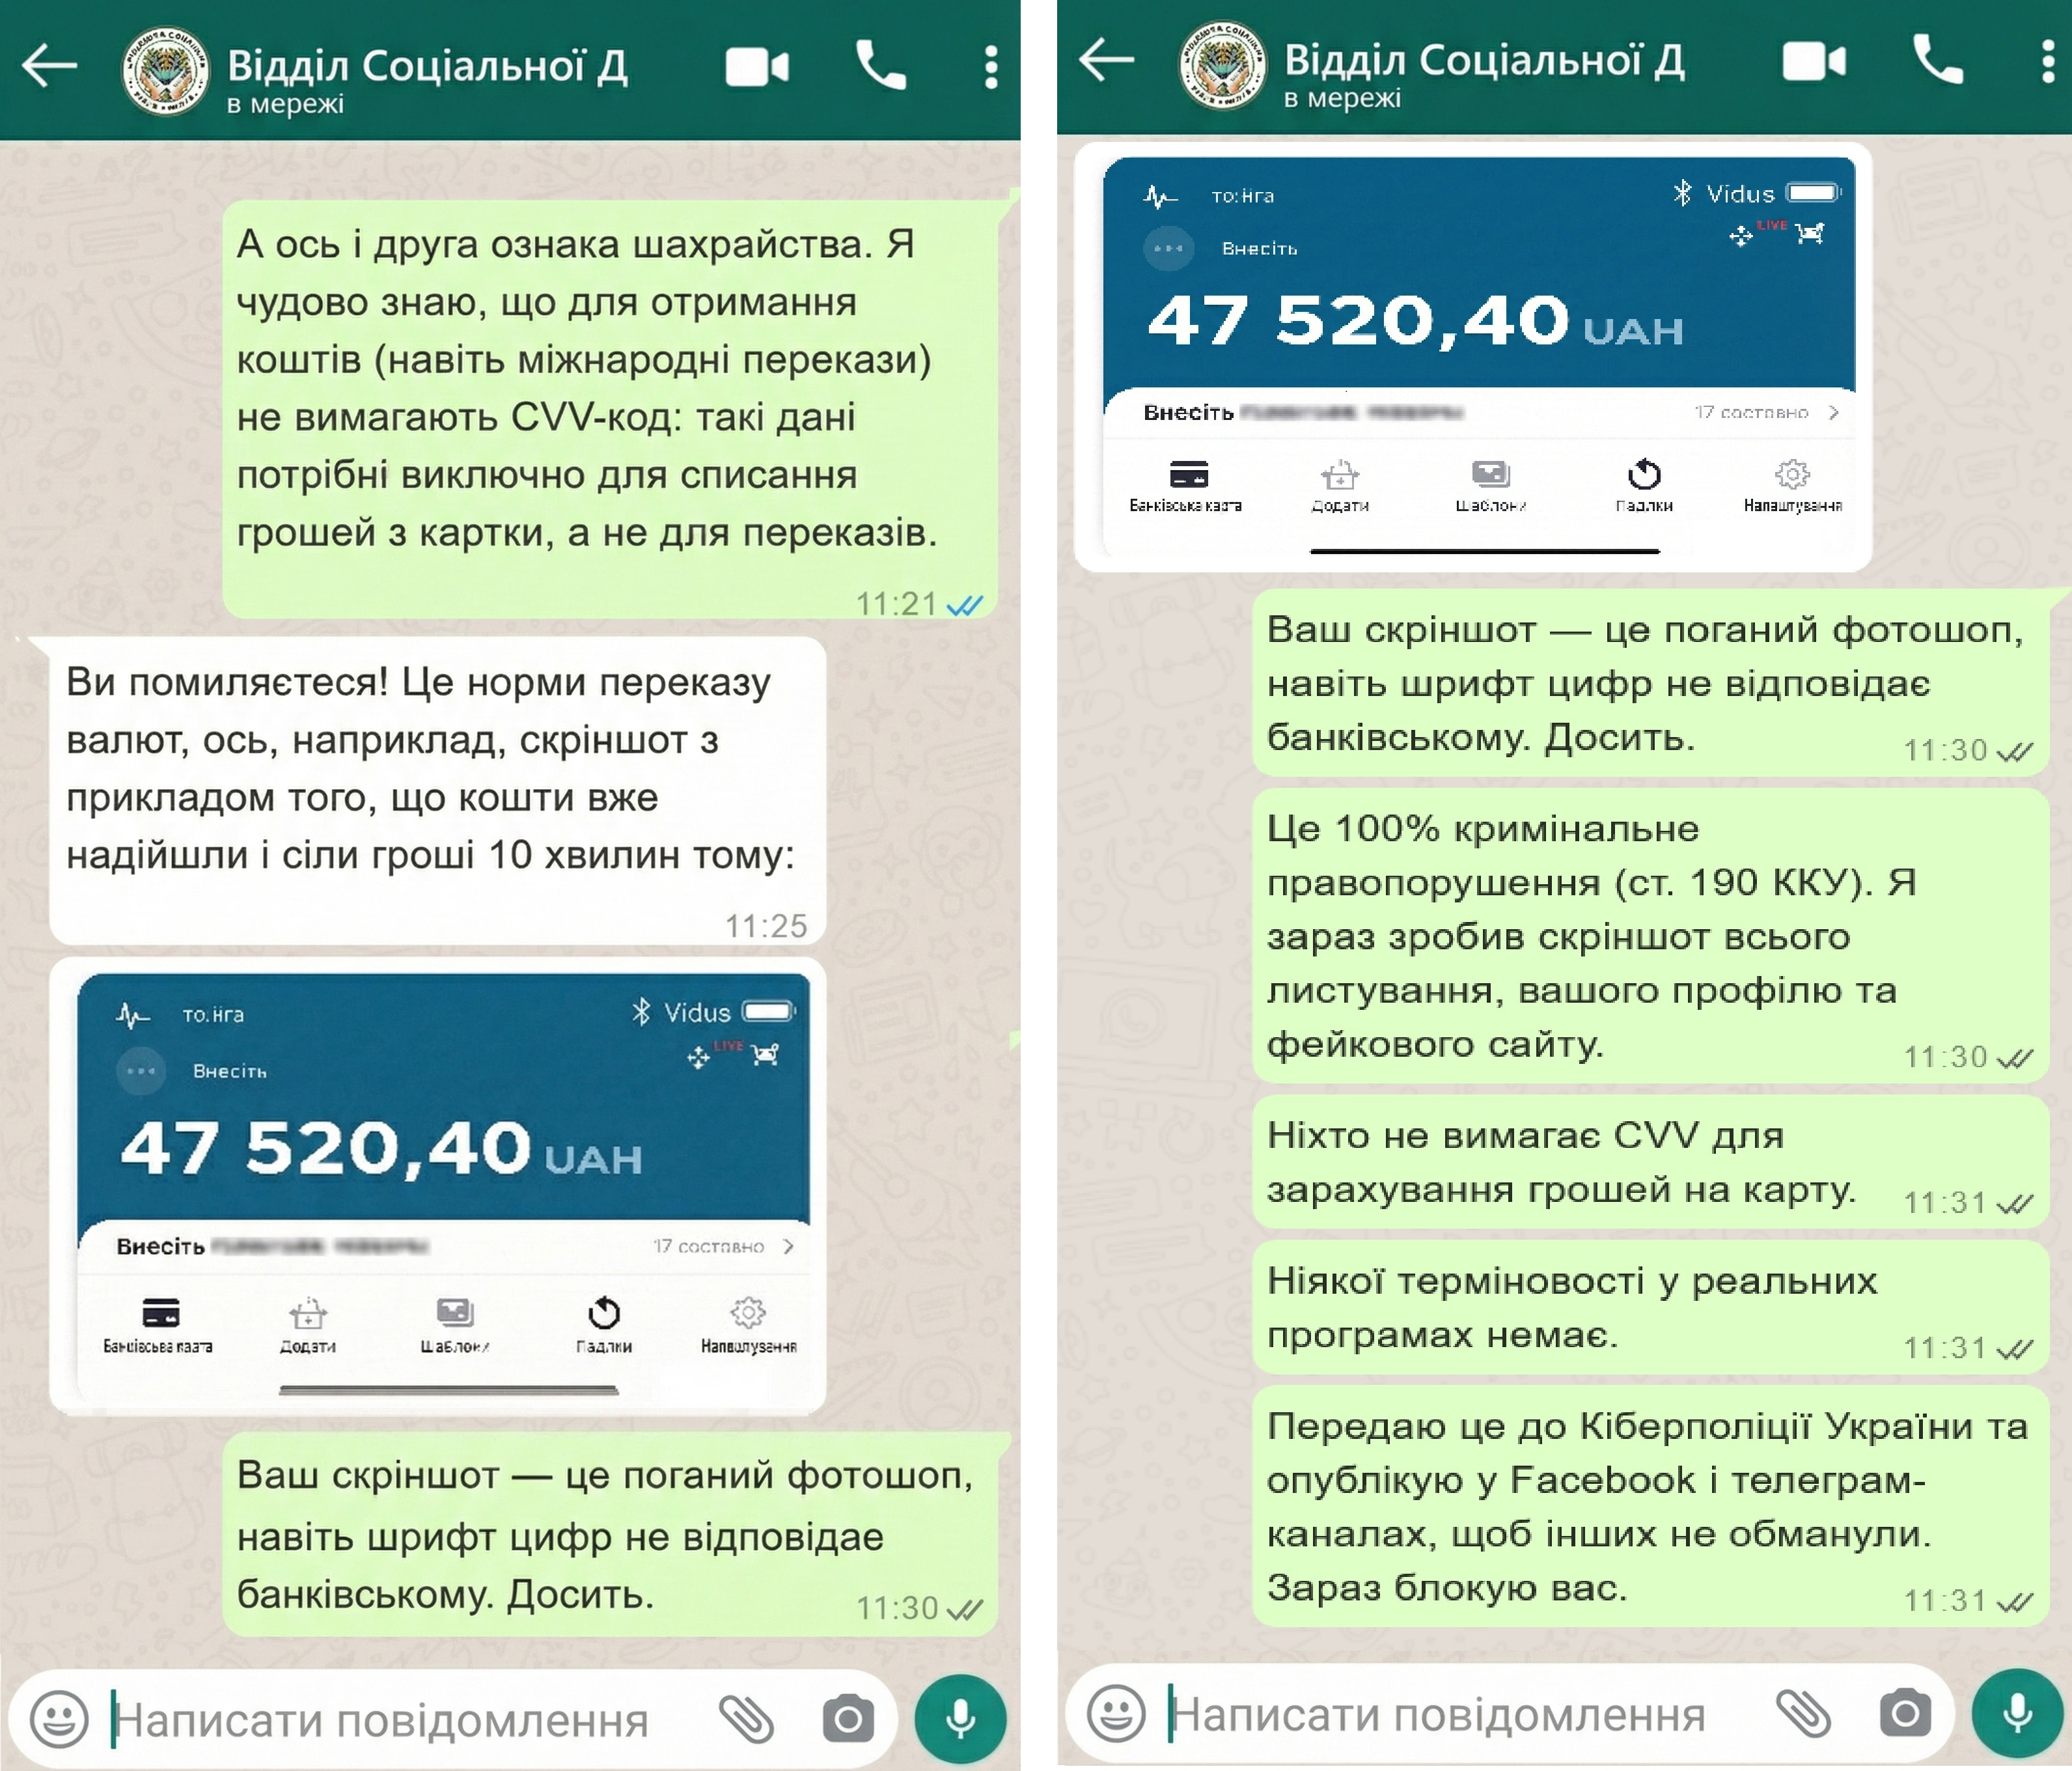
\includegraphics[width=0.75\linewidth]{img/figure6_16.jpg} 
    \caption{Листування з шахраєм}
    \label{fig:6_16}
\end{figure}

Як зрозуміти, що ваш смартфон під загрозою? Існує низка технічних та поведінкових індикаторів:

\begin{itemize}
    \item \textbf{Повільна робота, швидка розрядка та перегрів.}
    Наприклад, смартфон «гальмує» без причини, а батарея сідає набагато швидше, ніж зазвичай. Технічно це означає, що шкідливе ПЗ працює у фоні, постійно навантажуючи процесор або графічний чіп (наприклад, для прихованого майнінгу криптовалют чи участі в DDoS-атаках).

    \item \textbf{Поява незрозумілих додатків та іконок.}
    Наприклад, на робочому столі з’являються програми, які ви точно не встановлювали. Це пряма ознака того, що троян-завантажувач вже отримав контроль над системою і самостійно інсталює нові шкідливі модулі.

    \item \textbf{Несподівані зміни в налаштуваннях.}
    Наприклад, самовільно змінилася стартова сторінка в браузері, з'явилися невідомі розширення або додатки раптом отримали небезпечні дозволи (наприклад, доступ до «Спеціальних можливостей»), хоча ви їх не надавали.

    \item \textbf{Нав'язлива реклама та перенаправлення.}
    Наприклад, рекламні вікна з’являються хаотично, навіть поверх інших програм чи екрану блокування. Браузер може автоматично переходити на невідомі сайти. Це класична робота \textit{Adware} (рекламного ПЗ).

    \item \textbf{Аномалії з банківськими додатками та фінансами.}
    Наприклад, ви помічаєте SMS про дрібні списання чи транзакції, які ви не робили. Або ж справжній банківський додаток раптом блокується, і з'являється фальшиве вікно з вимогою повторно ввести пароль чи PIN-код («оверлей-атака»).

    \newpage

    \item \textbf{Скарги від друзів на спам.}
    Наприклад, ваші контакти у месенджерах чи пошті починають отримувати від вас дивні повідомлення з покликаннями. Це означає, що хробак чи троян вже використовує ваш акаунт та пристрій для подальшого поширення інфекції.

    \item \textbf{Підозріла активність камери, мікрофона та мережі.}
    Наприклад, індикатор камери чи мікрофона вмикається сам по собі, коли ви не використовуєте додатки. Також може фіксуватися аномально велике використання мобільних даних у фоновому режимі — це пристрій зв'язується з серверами зловмисників.
\end{itemize}

\textit{Якщо ви помітили одну або декілька з цих ознак, це вагомий привід негайно перевірити систему. Не ігноруйте ці сигнали, оскільки вони рідко виникають без причини.}

\subsection*{Як діяти в таких ситуаціях?}

\begin{enumerate}
    \item \textbf{Негайно відключіть пристрій від Інтернету} (Wi-Fi та мобільні дані), щоб зупинити передачу даних зловмисникам.
    \item \textbf{Перевірте останні встановлені додатки} та видаліть усе підозріле, що ви не встановлювали особисто.
    \item \textbf{Запустіть повне сканування} надійним мобільним антивірусом.
    \item \textbf{Перевірте дозволи} (особливо «Спеціальні можливості» та «Адміністратори пристрою») і відкличте їх у сумнівних програм.
    \item \textbf{Крайній захід.} Якщо нічого не допомагає — зробіть резервну копію важливих даних (лише фото, документи) та виконайте повне скидання до заводських налаштувань.
\end{enumerate}


\section{Методи перевірки безпеки програм}

Не встановлюйте програму одразу, особливо якщо вона отримана поза офіційним магазином. Будь-який застосунок (файл \texttt{.apk}, \texttt{.exe}) чи покликання з месенджера або пошти вимагає перевірки ще до запуску.

\textit{Алгоритм екстреної дії.} Якщо ви вже встановили щось підозріле, негайно відключіть пристрій від Інтернету (Wi-Fi, мобільні дані), щоб зупинити зв'язок із серверами зловмисників. Перезавантажте пристрій у «Безпечному режимі» (Safe Mode), перевірте список дозволів та видаліть програму.

Далі — три рівні перевірки за допомогою доступних ресурсів. Якщо бодай один пункт викликає сумнів — не встановлюйте програму.

\subsection*{1. Перевірка джерела та репутації (Хто автор?)}

\begin{itemize}
    \item \textbf{1.1. Офіційні магазини.} Встановлюйте програми переважно з офіційних джерел. Перевіряйте ім’я розробника, відгуки та кількість завантажень:
    \begin{itemize}
        \item Google Play: \url{https://play.google.com}
        \item Apple App Store: \url{https://apps.apple.com}
        \item Microsoft Store: \url{https://apps.microsoft.com/}
    \end{itemize}

    \item \textbf{1.2. Перевірка покликання (URL).} Перш ніж завантажувати файл, перевірте адресу:
    \begin{itemize}
        \item \textbf{VirusTotal} (перевіряє десятками антивірусів): \url{https://www.virustotal.com/}
        \item \textbf{URLScan} (показує, куди перенаправляється запит): \url{https://urlscan.io/}
        \item \textbf{PhishTank} (база фішингових сайтів): \url{https://www.phishtank.com}
    \end{itemize}

    \item \textbf{1.3. Перевірка домену.} Перевірте вік сайту. Шахрайські ресурси часто зареєстровані лише кілька днів тому:
    \begin{itemize}
        \item ICANN Lookup: \url{https://lookup.icann.org/}
        \item Whois: \url{https://www.whois.com/whois}
    \end{itemize}

    \item \textbf{1.4. Бази шахраїв.} Перевірка підозрілих сайтів, телефонів, карток:
    \begin{itemize}
        \item Сервіс Асоціації ЄМА: \url{https://www.stopfraud.com.ua}
        \item Кіберполіція: \url{https://ticket.cyberpolice.gov.ua}
        \item Перевірка посилань: \url{https://checkmylink.net/}
    \end{itemize}
\end{itemize}

\subsection*{2. Технічний аналіз файлу (До запуску)}

Якщо ви вже завантажили файл, але ще не запустили його:

\begin{itemize}
    \item \textbf{2.1. Статичний аналіз.} Завантажте файл на сервіс для сканування:
    \begin{itemize}
        \item VirusTotal (вкладка File): \url{https://www.virustotal.com/}
        \item Kaspersky OpenTip: \url{https://opentip.kaspersky.com/}
    \end{itemize}

    \item \textbf{2.2. Аналіз у пісочниці (Sandbox).} Спостереження за запуском у безпечному середовищі:
    \begin{itemize}
        \item ANY.RUN (інтерактивний аналіз): \url{https://any.run}
        \item Hybrid Analysis (Falcon Sandbox): \url{https://www.hybrid-analysis.com}
    \end{itemize}
    
    \item \textbf{2.3. Перевірка цифрового підпису.} Переконайтеся, що файл підписаний оригінальним розробником (використовуйте інструменти \texttt{apksigner} для Android або \texttt{codesign} для macOS).
\end{itemize}

\subsection*{3. Аналіз поведінки (Після встановлення)}

\begin{itemize}
    \item \textbf{3.1. Антивірусне сканування.}
    Використовуйте \textbf{Google Play Protect} (Android), \textbf{Windows Defender} (Windows) або сканери за вимогою (\textbf{Malwarebytes}, \textbf{ESET Online Scanner}).
    
    \item \textbf{3.2. Моніторинг активності.}
    Використовуйте інструменти на кшталт \textbf{TCPView} (для відстеження мережевих з'єднань) або \textbf{Process Explorer} (для виявлення прихованих процесів) із пакету Microsoft Sysinternals.
\end{itemize}

\section*{Висновки та рекомендації}

\textbf{Короткі правила безпеки:}
\begin{enumerate}
    \item Спершу перевірка на VirusTotal, потім — завантаження.
    \item Завантажуйте лише з офіційних магазинів.
    \item Сумнівні дозволи — ознака шахрайства (наприклад, «Ліхтарик» просить доступ до SMS).
    \item Не надавайте дозвіл на «Спеціальні можливості» (Accessibility) без абсолютної впевненості.
\end{enumerate}

\textbf{Важлива рекомендація.}
У контексті захисту від мобільного шахрайства критично важливою є перевірка джерела завантаження. Асоціація ЄМА наполегливо рекомендує перед переходом за покликаннями для завантаження файлів (особливо з невідомих джерел) здійснювати верифікацію URL-адреси через спеціалізований сервіс \textbf{CheckMyLink} (\url{https://check.ema.com.ua/}).

\newpage

Актуальність цього інструменту зумовлена поширенням банківських троянів, які маскуються під корисні утиліти або ігри. Використання сканера дозволяє виявити загрозу ще на етапі переходу за покликанням, попередивши завантаження шкідливого контенту та компрометацію платіжних даних користувача~\cite{EMA_CheckMyLink}.

Узагальнений підхід до верифікації програмного забезпечення, що поєднує автоматизований аналіз та ручну перевірку, представлено на рис.~\ref{fig:6_17}.

\begin{figure}[H]
    \centering
    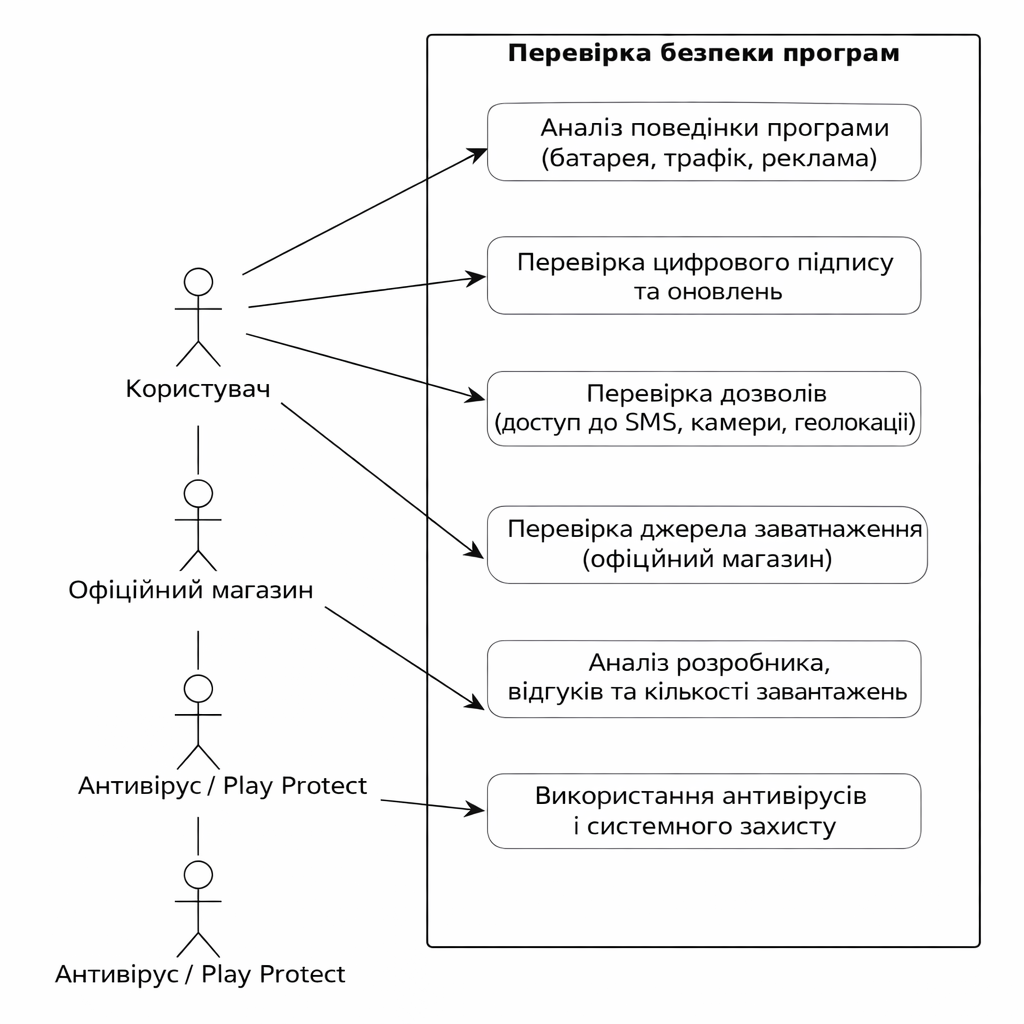
\includegraphics[width=0.95\linewidth]{img/figure6_17.png} 
    \caption{Методи перевірки безпеки програм}
    \label{fig:6_17}
\end{figure}

\section{Поради щодо безпечного завантаження програм}

Безпечне завантаження програм — це поєднання уважності, критичного мислення й дотримання простих правил цифрової гігієни. Дотримуючись їх, ви зменшите ризик інфікувати пристрій і запобігти більшості атак.

\begin{enumerate}
    \item \textbf{Завантажуйте тільки з офіційних магазинів.}
    Використовуйте Google Play, App Store або Microsoft Store. Ці магазини мають вбудовані механізми перевірки додатків (наприклад, Play Protect). Файли з розширенням \texttt{.apk} чи \texttt{.exe} зі сторонніх сайтів, форумів чи покликання з месенджерів несуть найвищий ризик зараження.

    \item \textbf{Користуйтеся захистом.}
    Встановіть надійний антивірус або захисний додаток (відомі продукти від ESET, Avast, Kaspersky тощо). Навіть вбудовані сервіси типу Play Protect допомагають виявляти підозрілі програми й блокувати небезпечні дії.

    \item \textbf{Перевіряйте розробника, відгуки та оновлення.}
    Перед натисканням кнопки «Встановити», перевірте видавця (чи це справді та компанія?), кількість завантажень (в оригіналу будуть мільйони, у підробки — тисячі) та відгуки (особливо негативні — шукайте скарги на шахрайство). Фейкові програми часто мають підозріло схожі назви. Також уникайте додатків, які не оновлювалися роками — вони можуть містити старі, але небезпечні вразливості.

    \newpage

    \item \textbf{Перевіряйте список дозволів.}
    Уважно дивіться, до чого програма хоче отримати доступ під час встановлення. 
  
    
    Якщо «Калькулятор» чи «Ліхтарик» вимагає доступу до ваших SMS, контактів, камери чи «Спеціальних можливостей» (\textit{Accessibility}) без очевидної на те причини — не встановлюйте такий додаток. Це майже завжди свідчить про небезпеку.

    \item \textbf{Не ігноруйте попередження системи.}
    Легальні програми мають дійсний сертифікат (цифровий підпис) розробника. Якщо під час встановлення система (особливо на Android чи Windows) попереджає, що підпис невідомий або недійсний, від інсталяції слід категорично відмовитися.

    \item \textbf{Після встановлення контролюйте поведінку пристрою.}
    Звертайте увагу на різке падіння автономності, перегрів, уповільнення роботи, раптову появу реклами або автоматичні перенаправлення в браузері.

    \item \textbf{Використовуйте постійний захист (Антивірус).}
    Встановіть надійне захисне рішення. Навіть вбудовані засоби (як Google Play Protect чи Windows Defender) аналізують поведінку програм у фоновому режимі і блокують ті, що намагаються зв'язатися зі шкідливими серверами або виконати небезпечні дії.
\end{enumerate}

\newpage

\subsection*{Що робити, якщо ви встановили підозрілий додаток?}

Якщо ви виявили комп'ютерний вірус, ви можете відчути гнів, сором або страх. Це нормальні реакції. Зробіть паузу, глибоко вдихніть і зробіть максимально повільний, тривалий видих. Це фізіологічно знизить рівень паніки. Ваша безпека зараз залежить від спокійних, алгоритмічних дій. Ви не зробили нічого поганого — ви стали об’єктом професійної атаки.



\begin{enumerate}
    \item \textbf{Негайно видаліть} цей застосунок через налаштування телефону.
    
    \item \textbf{Перезавантажте пристрій у «Безпечному режимі» (Safe Mode)}, якщо програма не видаляється, і спробуйте видалити її звідти.
    \item \textbf{Проскануйте систему} надійним мобільним антивірусом.
    \item \textbf{Негайно змініть паролі} у банківських додатках, пошті та інших важливих сервісах.
    
    \item \textbf{По-можливості, фіксуйте підозрілі запити} (скріншоти, назву дозволу) для подальшого звернення до служби підтримки платформи або розробника.
\end{enumerate}

\vspace{0.3cm}
\textit{Краще кілька хвилин витратити на перевірку джерела, ніж потім втратити гроші чи доступ до особистих даних через поспішне встановлення.}

%\vspace{0.3cm}

\newpage

\section*{Висновки до розділу} 
\addcontentsline{toc}{section}{Висновки до розділу}

\begin{center}
    \textit{Смартфон — це центр управління життям у цифровому світі.}
\end{center}

Захист смартфона — це не про страх, а про свідому турботу про свій цифровий простір. Мета цієї книги — надати вам інструменти, які допоможуть відчувати впевненість, а не тривогу. Розуміння механізмів роботи шкідливого ПЗ та знання основних схем маніпуляцій формують вашу персональну «цифрову імунну систему», яка дозволяє користуватися технологіями вільно та безпечно.



Смартфон перестав бути просто засобом зв'язку; він перетворився на цифровий ключ до ваших фінансів, особистого листування та ідентичності. Саме тому встановлення додатків виключно з офіційних джерел та свідомий контроль дозволів є не обмеженням вашої свободи, а професійним підходом до експлуатації ґаджета.

Важливо пам’ятати, що регулярне оновлення програмного забезпечення — це передусім спосіб закрити технічні вразливості, на які полюють кіберзлочинці. Ваша уважність до оновлень та встановлення надійного пароля блокування екрана значно підвищують рівень захищеності ваших даних. Ставтеся до свого смартфона як до цінного ресурсу, що потребує відповідального ставлення, — це дозволить вам залишатися господарем власної цифрової ідентичності.

\textit{\textbf{Технічна підтримка доступна.} Якщо ви підозрюєте компрометацію даних або ваш пристрій зазнав атаки — не панікуйте. Пам’ятайте, що навіть досвідчені користувачі можуть стати ціллю професійної атаки. Автор готовий надати технічну консультацію та рекомендації щодо подальших дій. Своєчасна реакція є ключем до мінімізації будь-яких ризиків.}


